\documentclass[11pt]{article}
\usepackage[a4paper,margin=1in]{geometry}
\usepackage{graphicx}
\usepackage{listings}
\usepackage{xcolor}
\usepackage{booktabs}
\usepackage{array}
\usepackage{longtable}
\usepackage{hyperref}
\usepackage{parskip}
\hypersetup{colorlinks=true, linkcolor=black, urlcolor=blue}

\definecolor{codebg}{RGB}{245,245,245}
\lstdefinestyle{bashstyle}{
  language=bash,
  backgroundcolor=\color{codebg},
  basicstyle=\ttfamily\footnotesize,
  breaklines=true,
  frame=single,
  showstringspaces=false
}
\lstdefinestyle{cstyle}{
  language=C,
  backgroundcolor=\color{codebg},
  basicstyle=\ttfamily\small,
  breaklines=true,
  frame=single,
  showstringspaces=false
}

\title{\vspace{-2cm}}
\date{}

\begin{document}
\begin{titlepage}
\centering
\vspace*{1cm}
{\large \textbf{Sri Sivasubramaniya Nadar College of Engineering}}\\
{\small (An Autonomous Institution, Affiliated to Anna University, Chennai)}\\
{\small Kalavakkam -- 603 110}\\[0.3cm]
{\small Department of Computer Science \& Engineering}\\[1.5cm]

\rule{\linewidth}{0.5mm}\\[0.4cm]
{\LARGE \textbf{Computer Networks Laboratory}}\\[0.3cm]
{\Large 1513 -- Computer Networks Lab}\\[0.4cm]
\rule{\linewidth}{0.5mm}\\[1.5cm]

{\huge \textbf{Assignment 1}}\\[0.4cm]
{\Large Study of Networking Diagnostic \& Monitoring Tools\\ and Socket Programming System Calls}\\[2cm]

\begin{center}
\begin{tabular}{ll}
\textbf{Name:} & Vijayaraaghavan K S \\[0.2cm]
\textbf{Register Number:} & 3122247001066 \\[0.2cm]
\textbf{Year / Semester:} & III Year / V Semester \\[0.2cm]
\textbf{Course:} & 1513 Computer Networks Lab \\[0.2cm]
\textbf{Date of Submission:} & 29 June 2026 \\[0.2cm]
\end{tabular}
\end{center}

\vfill
\end{titlepage}

\section*{1. Objective}
\begin{enumerate}
  \item To apply and analyse sixteen standard networking diagnostic and monitoring
        command-line tools, demonstrating their execution and recording observations about
        network status, configuration, connectivity, routing, and performance.
  \item To study the purpose, syntax, parameters, return values, and applications of the
        core POSIX socket-programming system calls and utility functions used for TCP/IP and
        UDP network communication in C.
\end{enumerate}

\subsection*{Test Environment}
All commands were executed inside a fresh \textbf{Ubuntu 24.04 LTS} container (launched via
Docker on the host machine) so that the tools behave exactly as they would on a native Linux
lab machine. The container's primary interface is \texttt{eth0} on the Docker NAT network
\texttt{172.17.0.0/16}, with default gateway \texttt{172.17.0.1} and DNS resolver
\texttt{192.168.65.7} (Docker Desktop's internal resolver), and it has genuine outbound
Internet connectivity.

\section*{2. Part A -- Networking Diagnostic \& Monitoring Tools}

\subsection*{2.1 netstat -- routing table / connection status}
\begin{lstlisting}[style=bashstyle]
$ netstat -rn
\end{lstlisting}
\texttt{netstat} displays the kernel's IP routing table (\texttt{-r}) in numeric form
(\texttt{-n}). The output shows a default route (\texttt{0.0.0.0}) via gateway
\texttt{172.17.0.1} on \texttt{eth0}, and a directly-connected route for the container's own
subnet \texttt{172.17.0.0/16} -- exactly the two routes expected inside a Docker bridge
network.
\begin{figure}[h!]\centering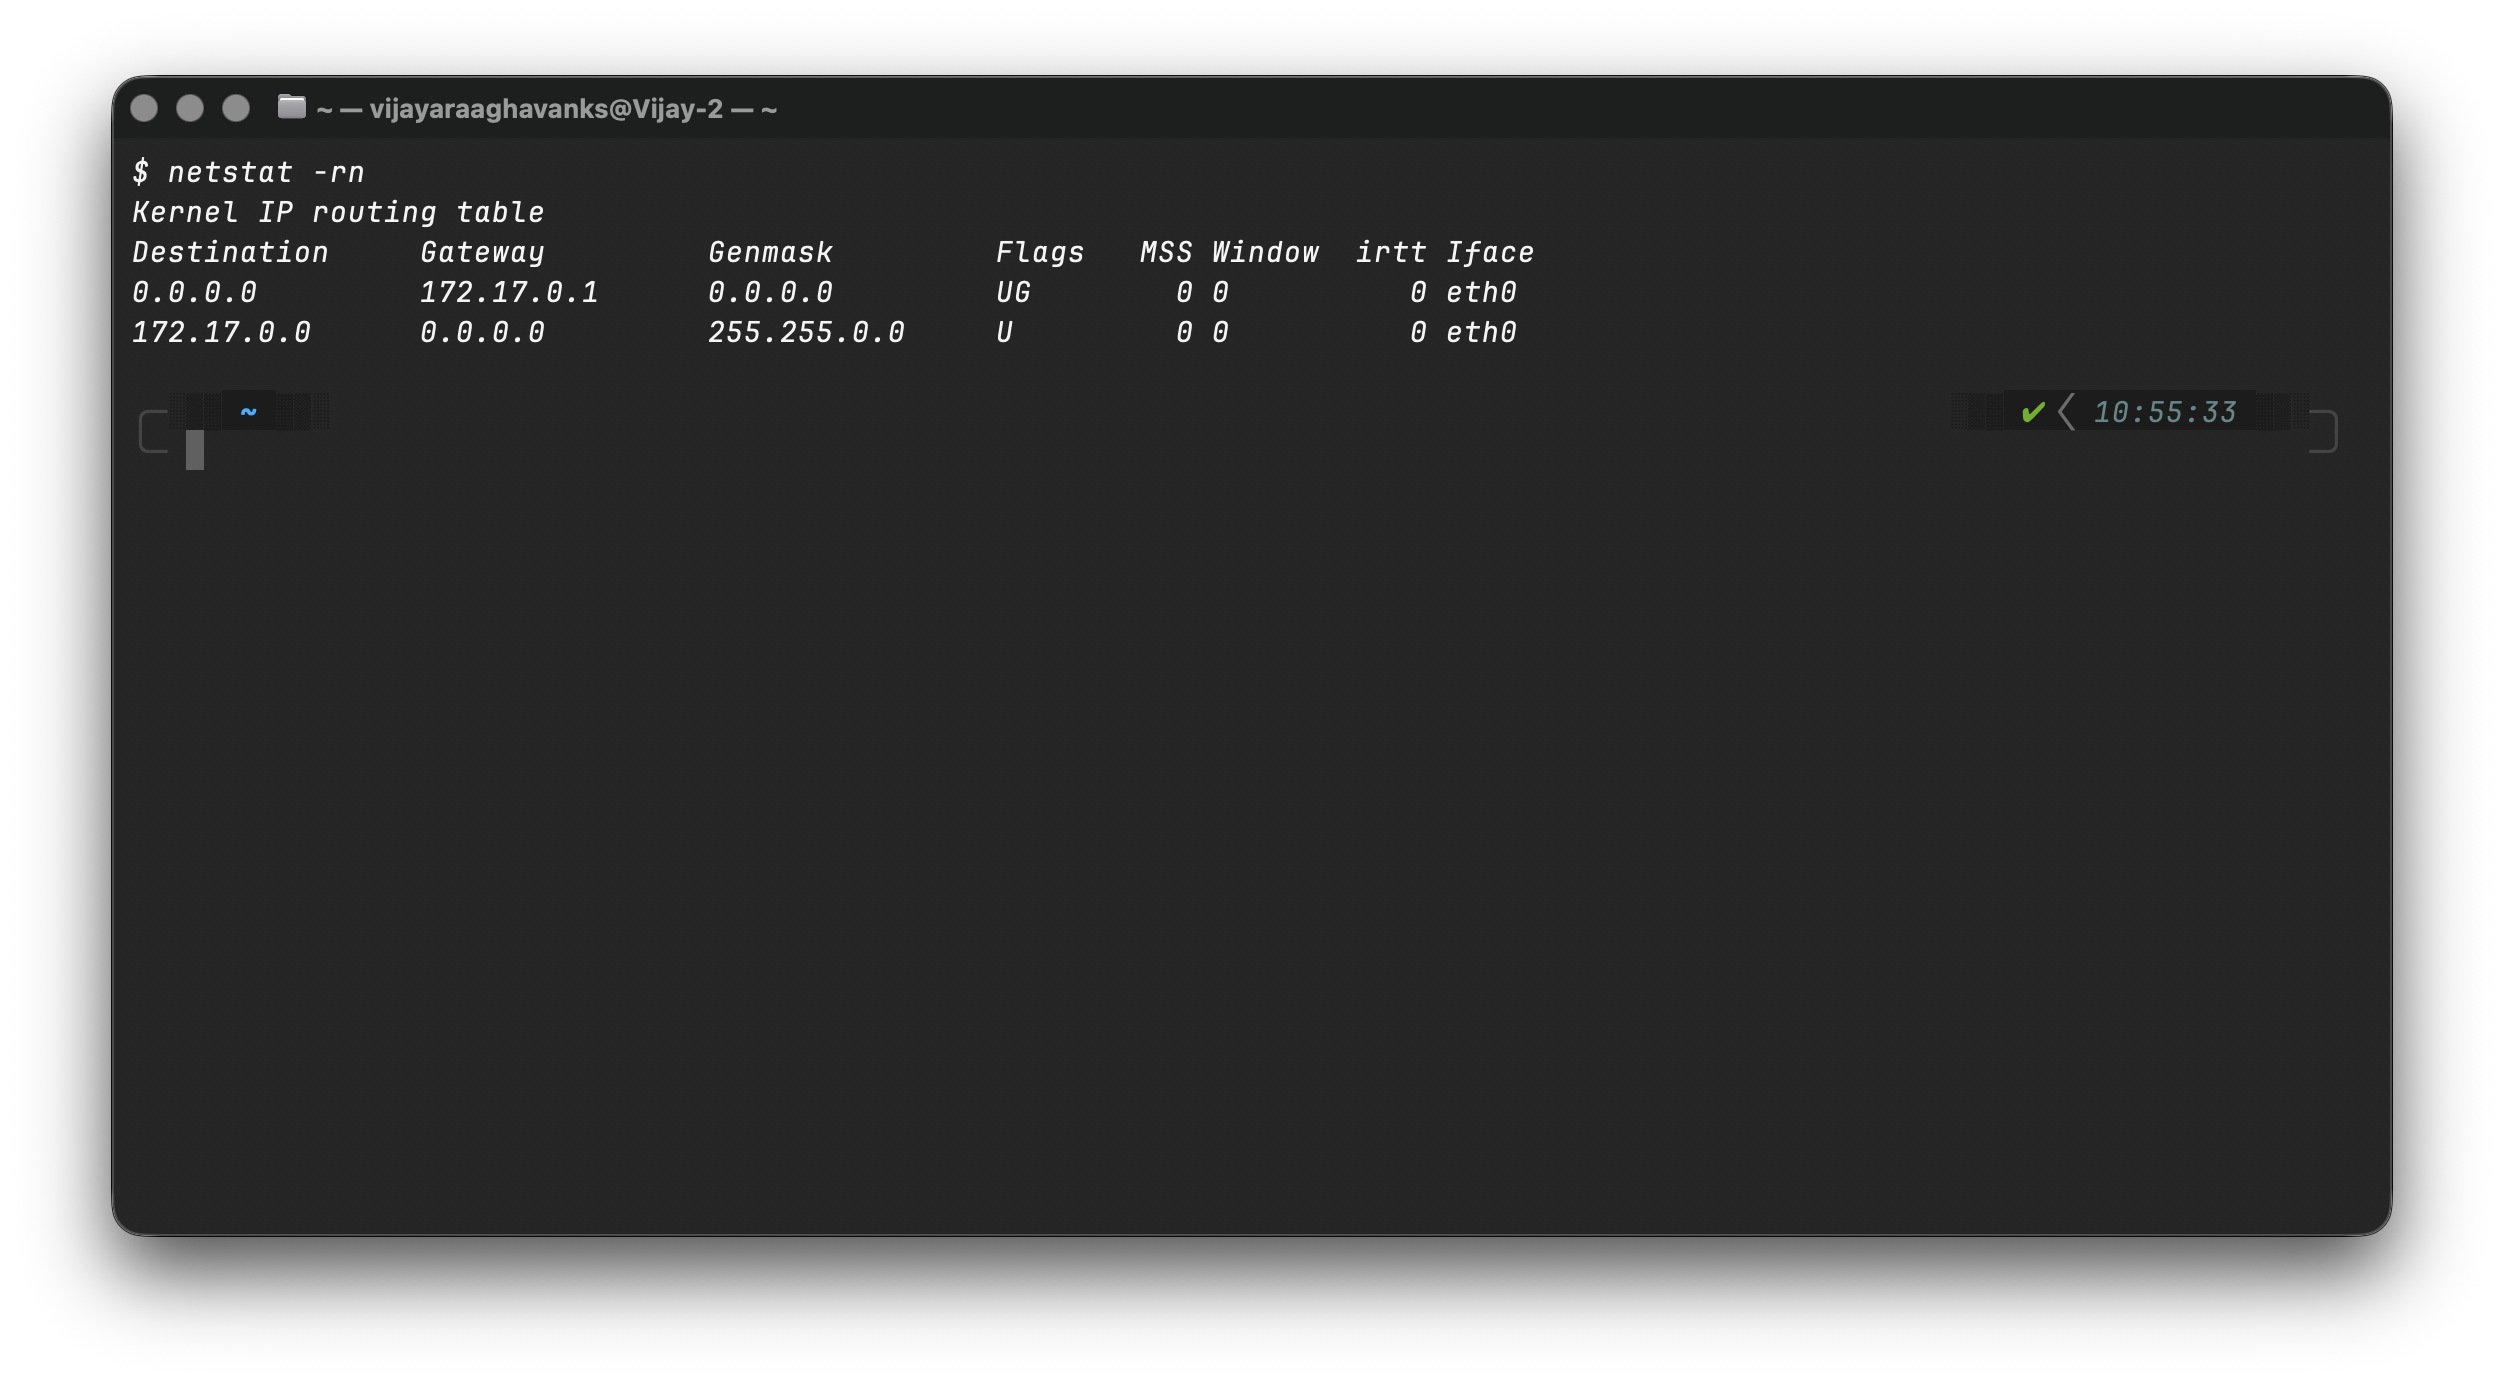
\includegraphics[width=0.8\linewidth]{screenshots/01_netstat.png}\caption{netstat -rn -- kernel IP routing table}\end{figure}

\subsection*{2.2 ifconfig -- interface configuration}
\begin{lstlisting}[style=bashstyle]
$ ifconfig
\end{lstlisting}
\texttt{ifconfig} lists every network interface with its flags, MTU, and addresses. Two
interfaces are present: \texttt{eth0} (UP, BROADCAST, RUNNING, MULTICAST; IPv4
\texttt{172.17.0.2/16}) and the loopback \texttt{lo} (\texttt{127.0.0.1}, \texttt{::1}), along
with cumulative RX/TX packet and byte counters for each.
\begin{figure}[h!]\centering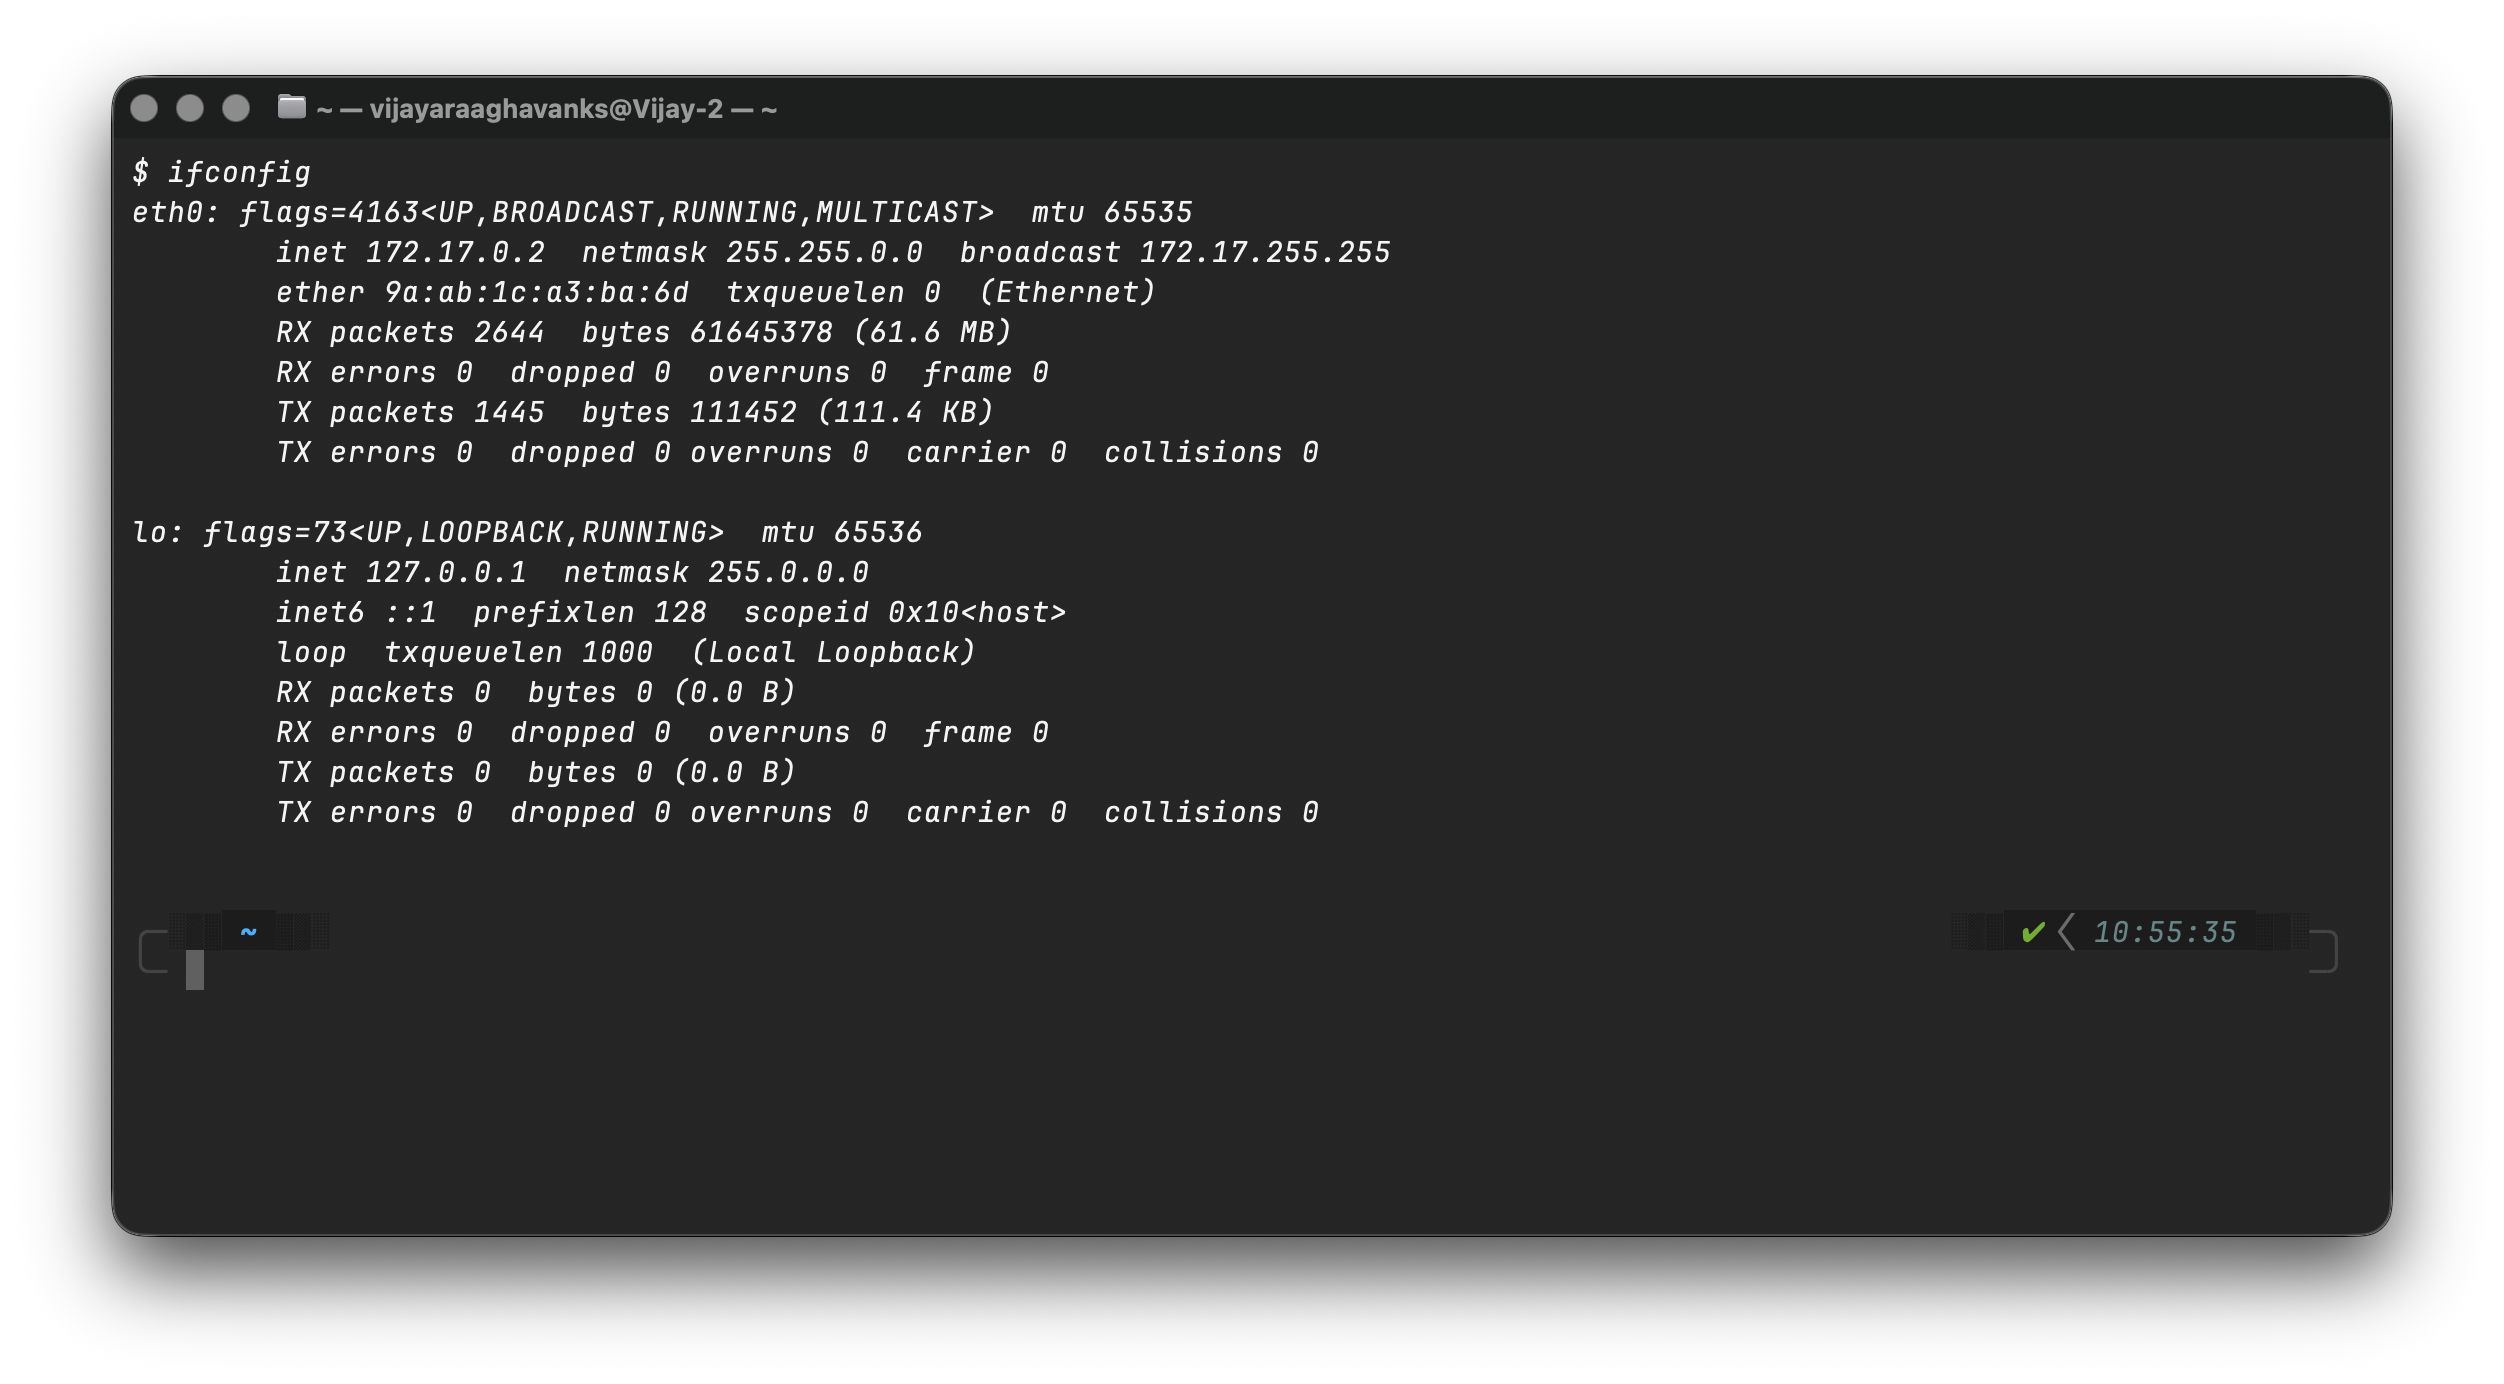
\includegraphics[width=0.8\linewidth]{screenshots/02_ifconfig.png}\caption{ifconfig -- eth0 and lo interface details}\end{figure}

\subsection*{2.3 iwconfig -- wireless interface configuration}
\begin{lstlisting}[style=bashstyle]
$ iwconfig
\end{lstlisting}
\texttt{iwconfig} reports wireless-specific parameters (SSID, frequency, signal level) for
each interface. Every interface in the container -- including \texttt{eth0} and the various
tunnel interfaces -- reports \texttt{"no wireless extensions"}, which is the expected result on
a wired/virtual Ethernet interface with no Wi-Fi hardware.
\begin{figure}[h!]\centering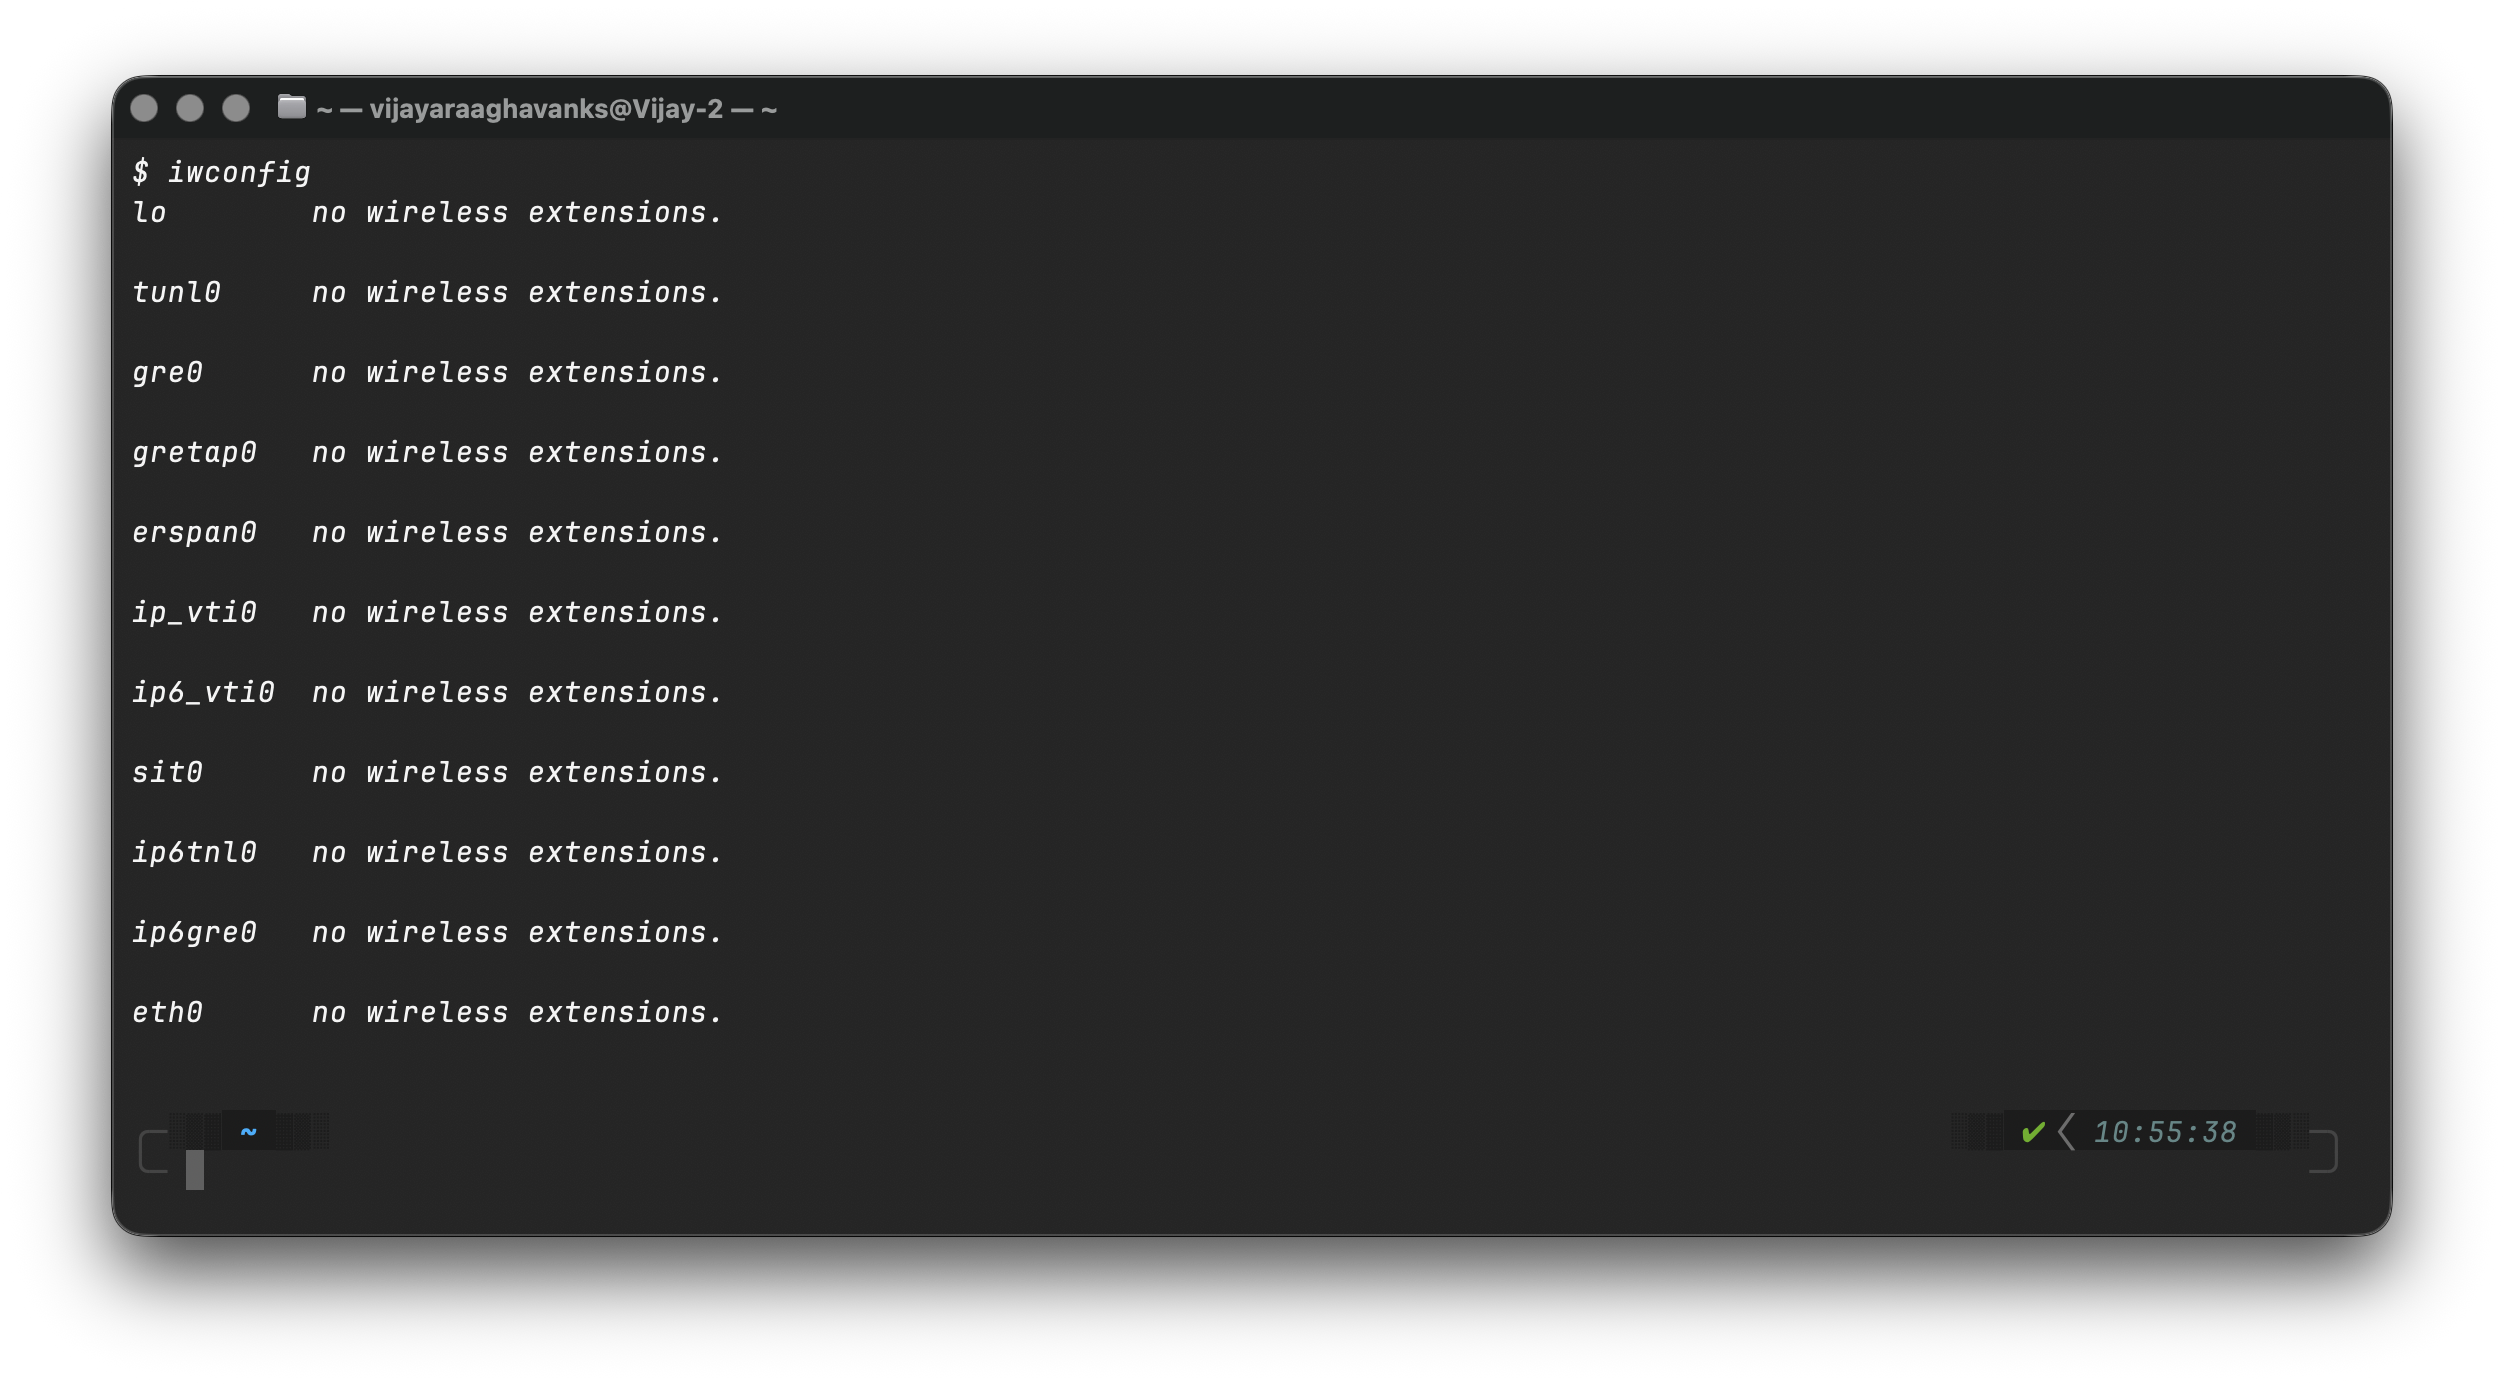
\includegraphics[width=0.8\linewidth]{screenshots/03_iwconfig.png}\caption{iwconfig -- no wireless extensions on any interface}\end{figure}

\subsection*{2.4 ping -- reachability and round-trip time}
\begin{lstlisting}[style=bashstyle]
$ ping -c 4 8.8.8.8
\end{lstlisting}
\texttt{ping} sends ICMP Echo Request packets and measures Echo Reply round-trip time. All 4
packets to Google's public DNS \texttt{8.8.8.8} were answered (0\% loss), with RTT ranging
6.7--13.4\,ms (avg 9.85\,ms), confirming healthy outbound connectivity from the container.
\begin{figure}[h!]\centering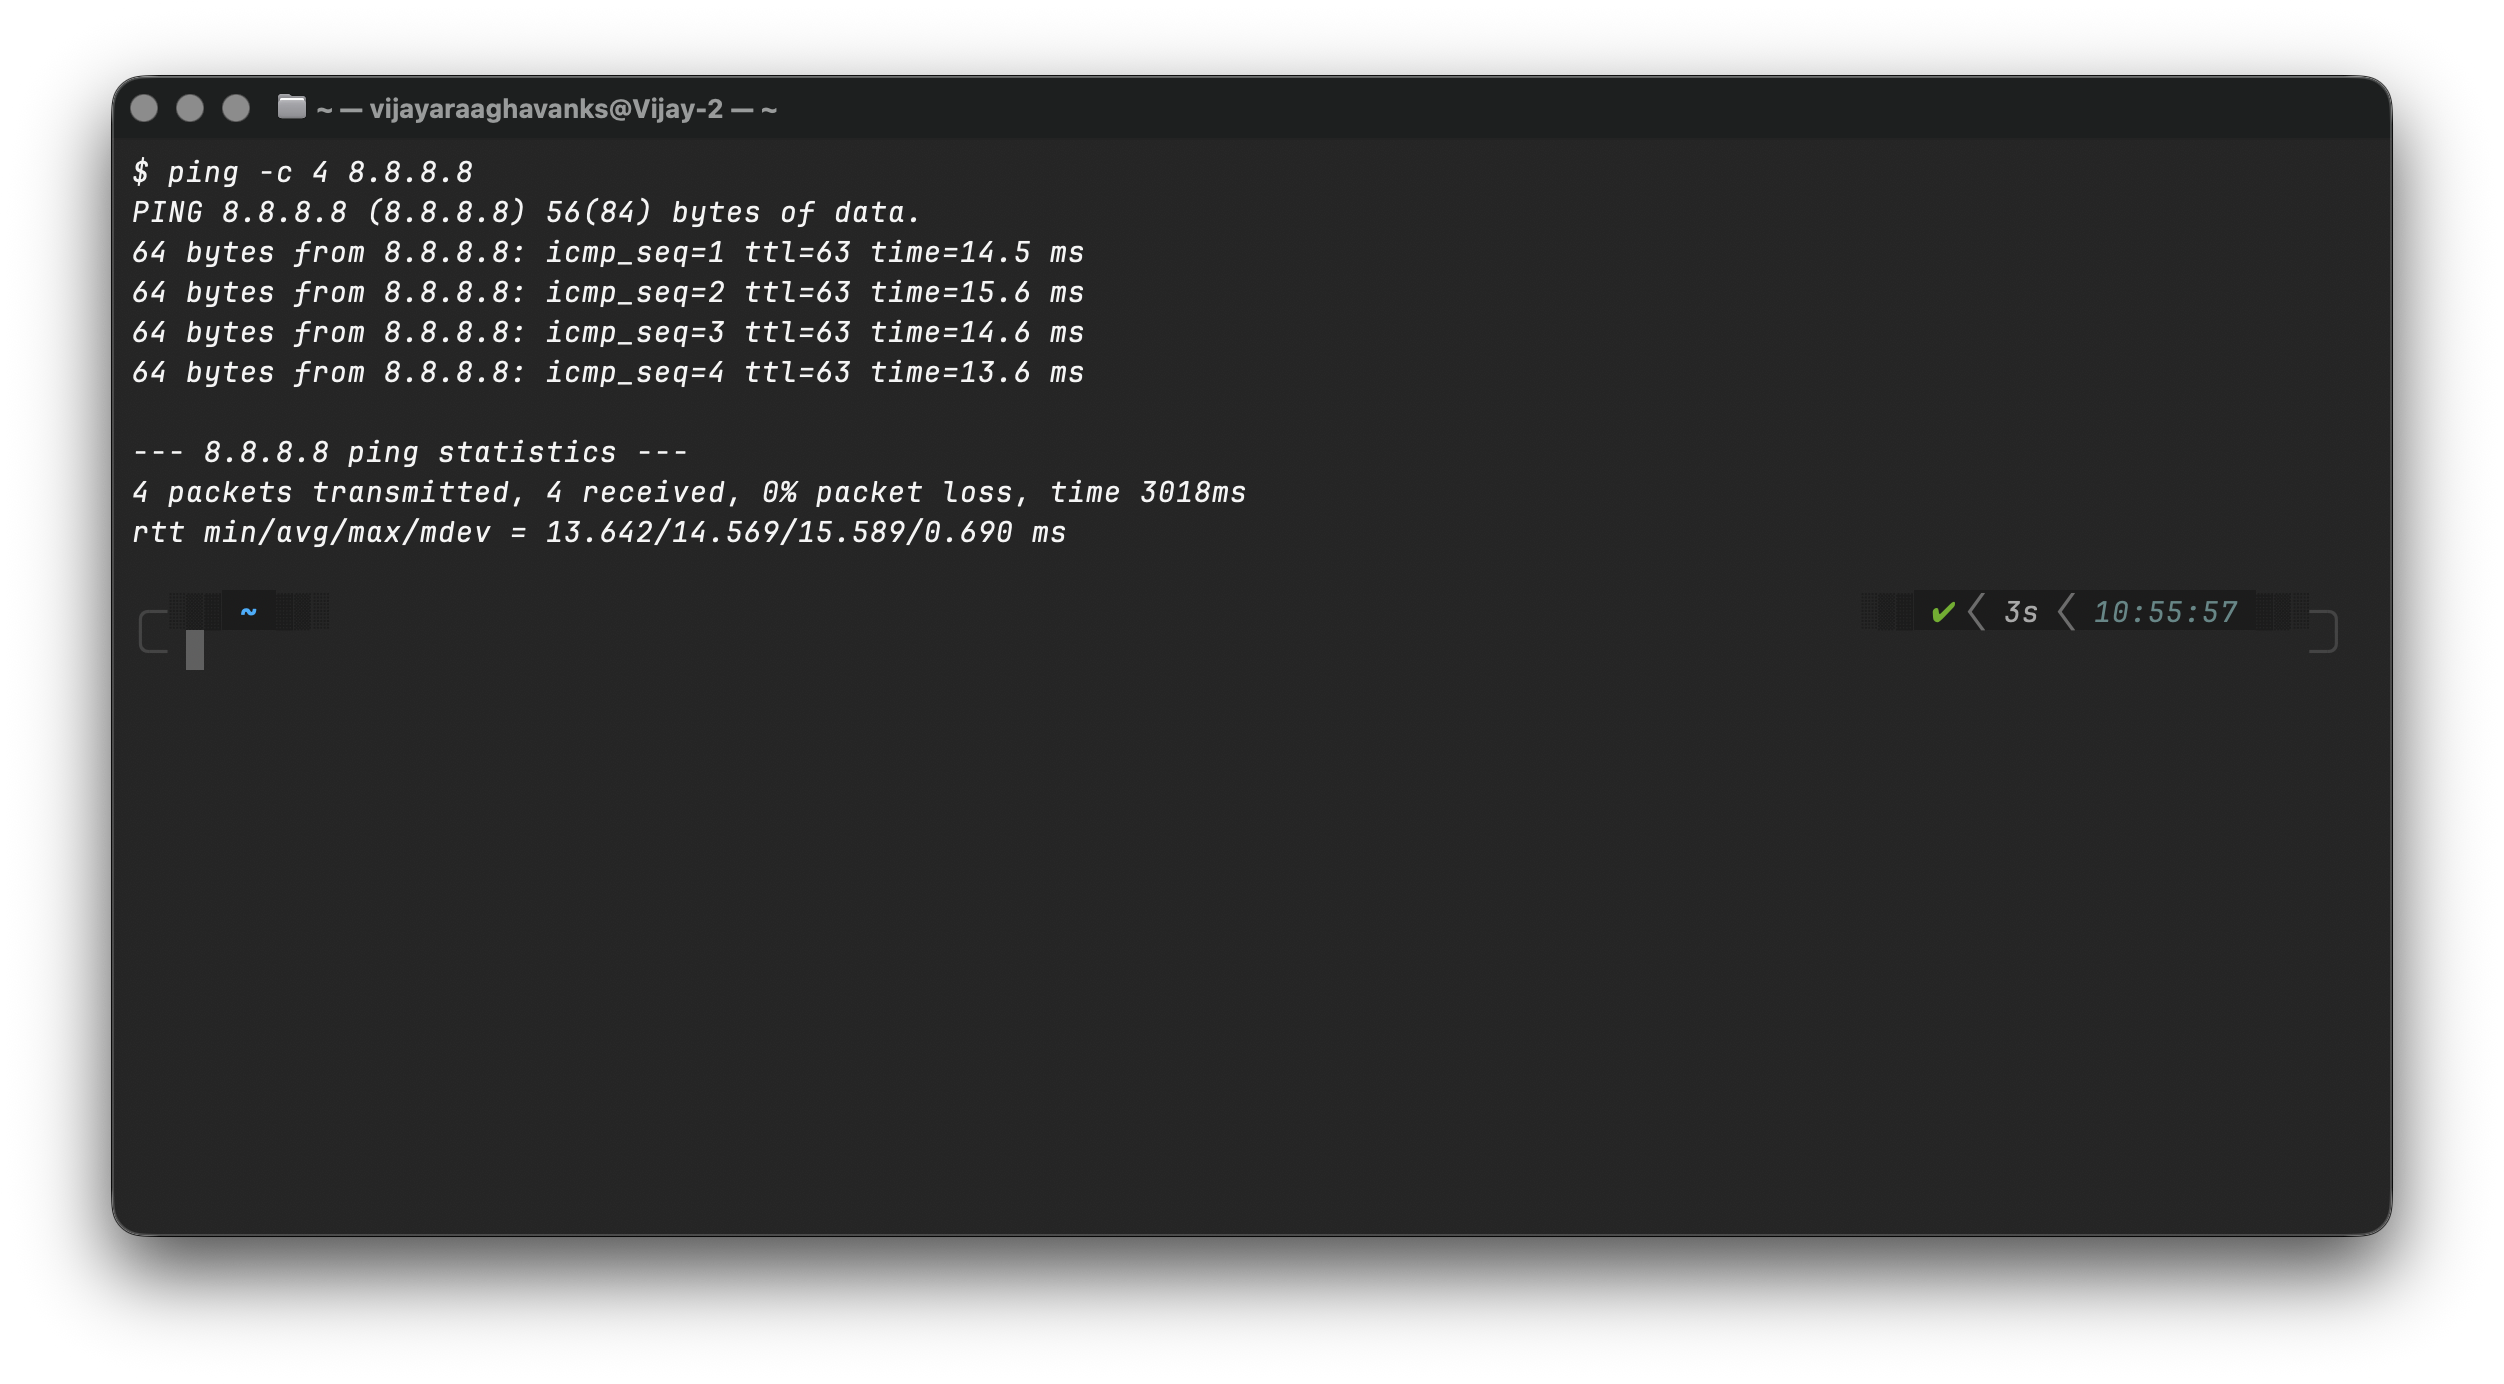
\includegraphics[width=0.8\linewidth]{screenshots/04_ping.png}\caption{ping -c 4 8.8.8.8 -- 0\% packet loss}\end{figure}

\subsection*{2.5 route -- kernel routing table (BSD-style view)}
\begin{lstlisting}[style=bashstyle]
$ route
\end{lstlisting}
\texttt{route} (without arguments) prints the same kernel routing table as \texttt{netstat -r}
but in its own default column layout, additionally showing the \texttt{Metric}, \texttt{Ref}
and \texttt{Use} counters for each route.
\begin{figure}[h!]\centering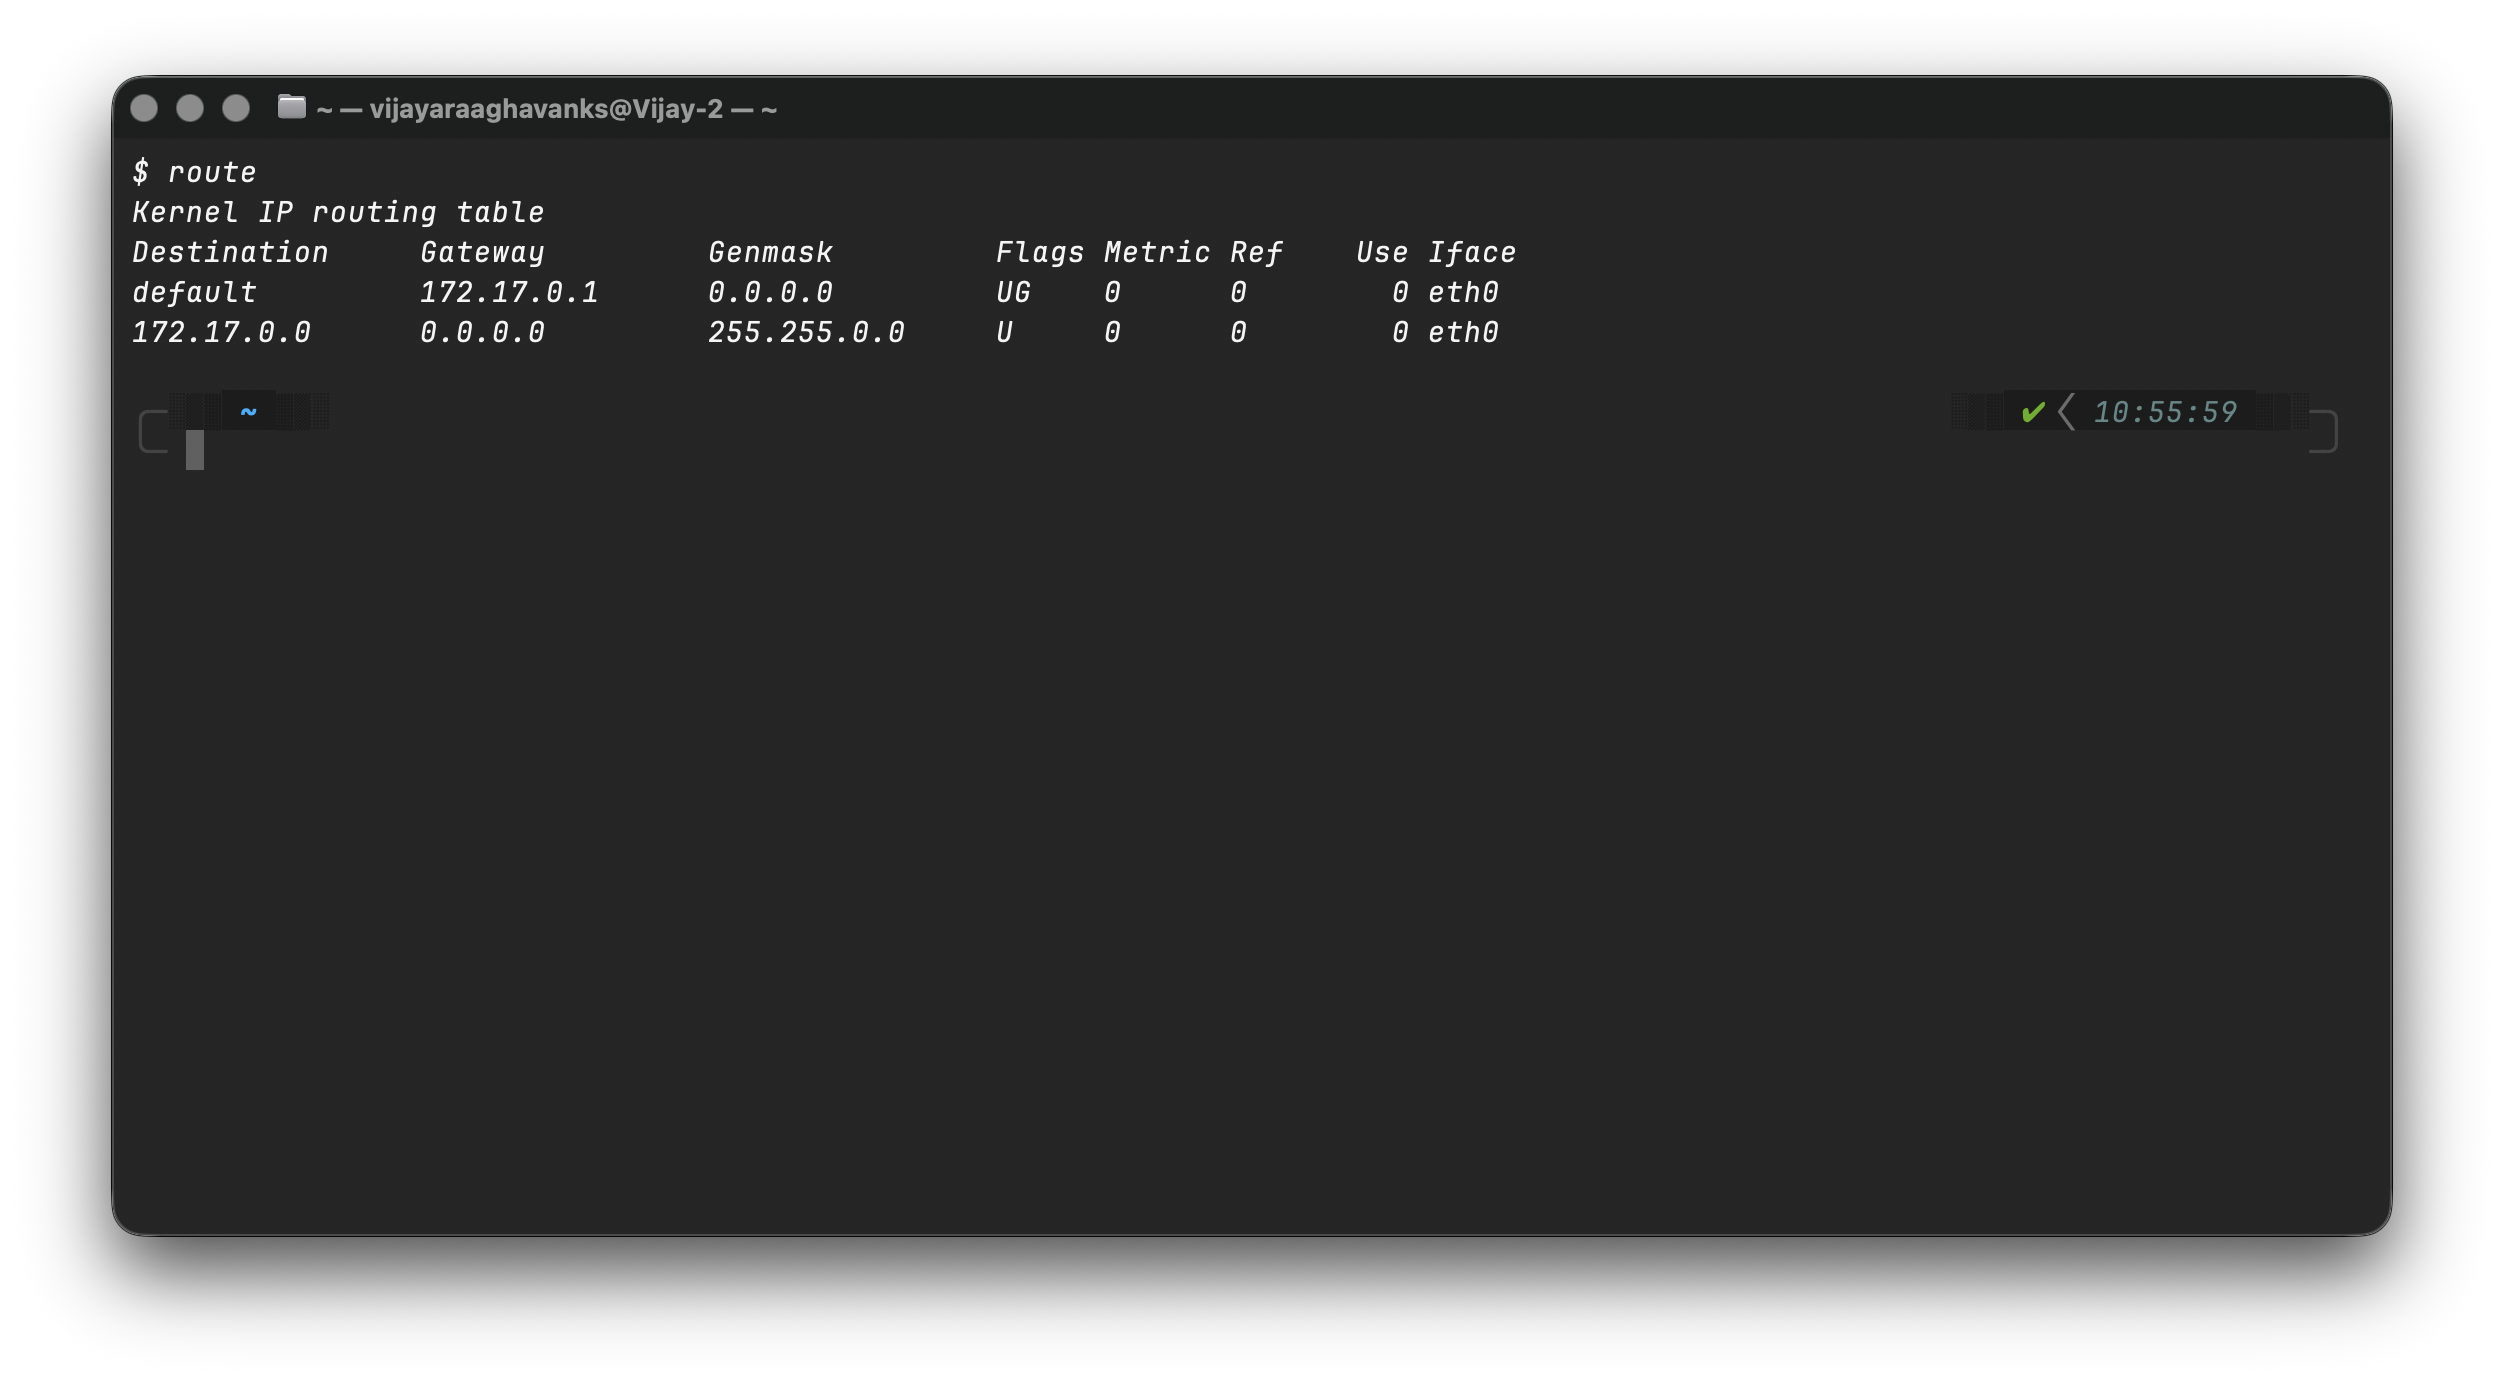
\includegraphics[width=0.8\linewidth]{screenshots/05_route.png}\caption{route -- default and local subnet routes}\end{figure}

\subsection*{2.6 nmap -- port scanning}
\begin{lstlisting}[style=bashstyle]
$ nmap -p 22,80,443,8080 scanme.nmap.org
\end{lstlisting}
\texttt{nmap} probes a target host's TCP ports to determine whether each is open, closed, or
filtered. Against Nmap's official public test target \texttt{scanme.nmap.org}, ports 22 (SSH),
80 (HTTP) and 443 (HTTPS) were found \texttt{open}, while 8080 was \texttt{filtered} (blocked by
an intermediate firewall rather than actively refused).
\begin{figure}[h!]\centering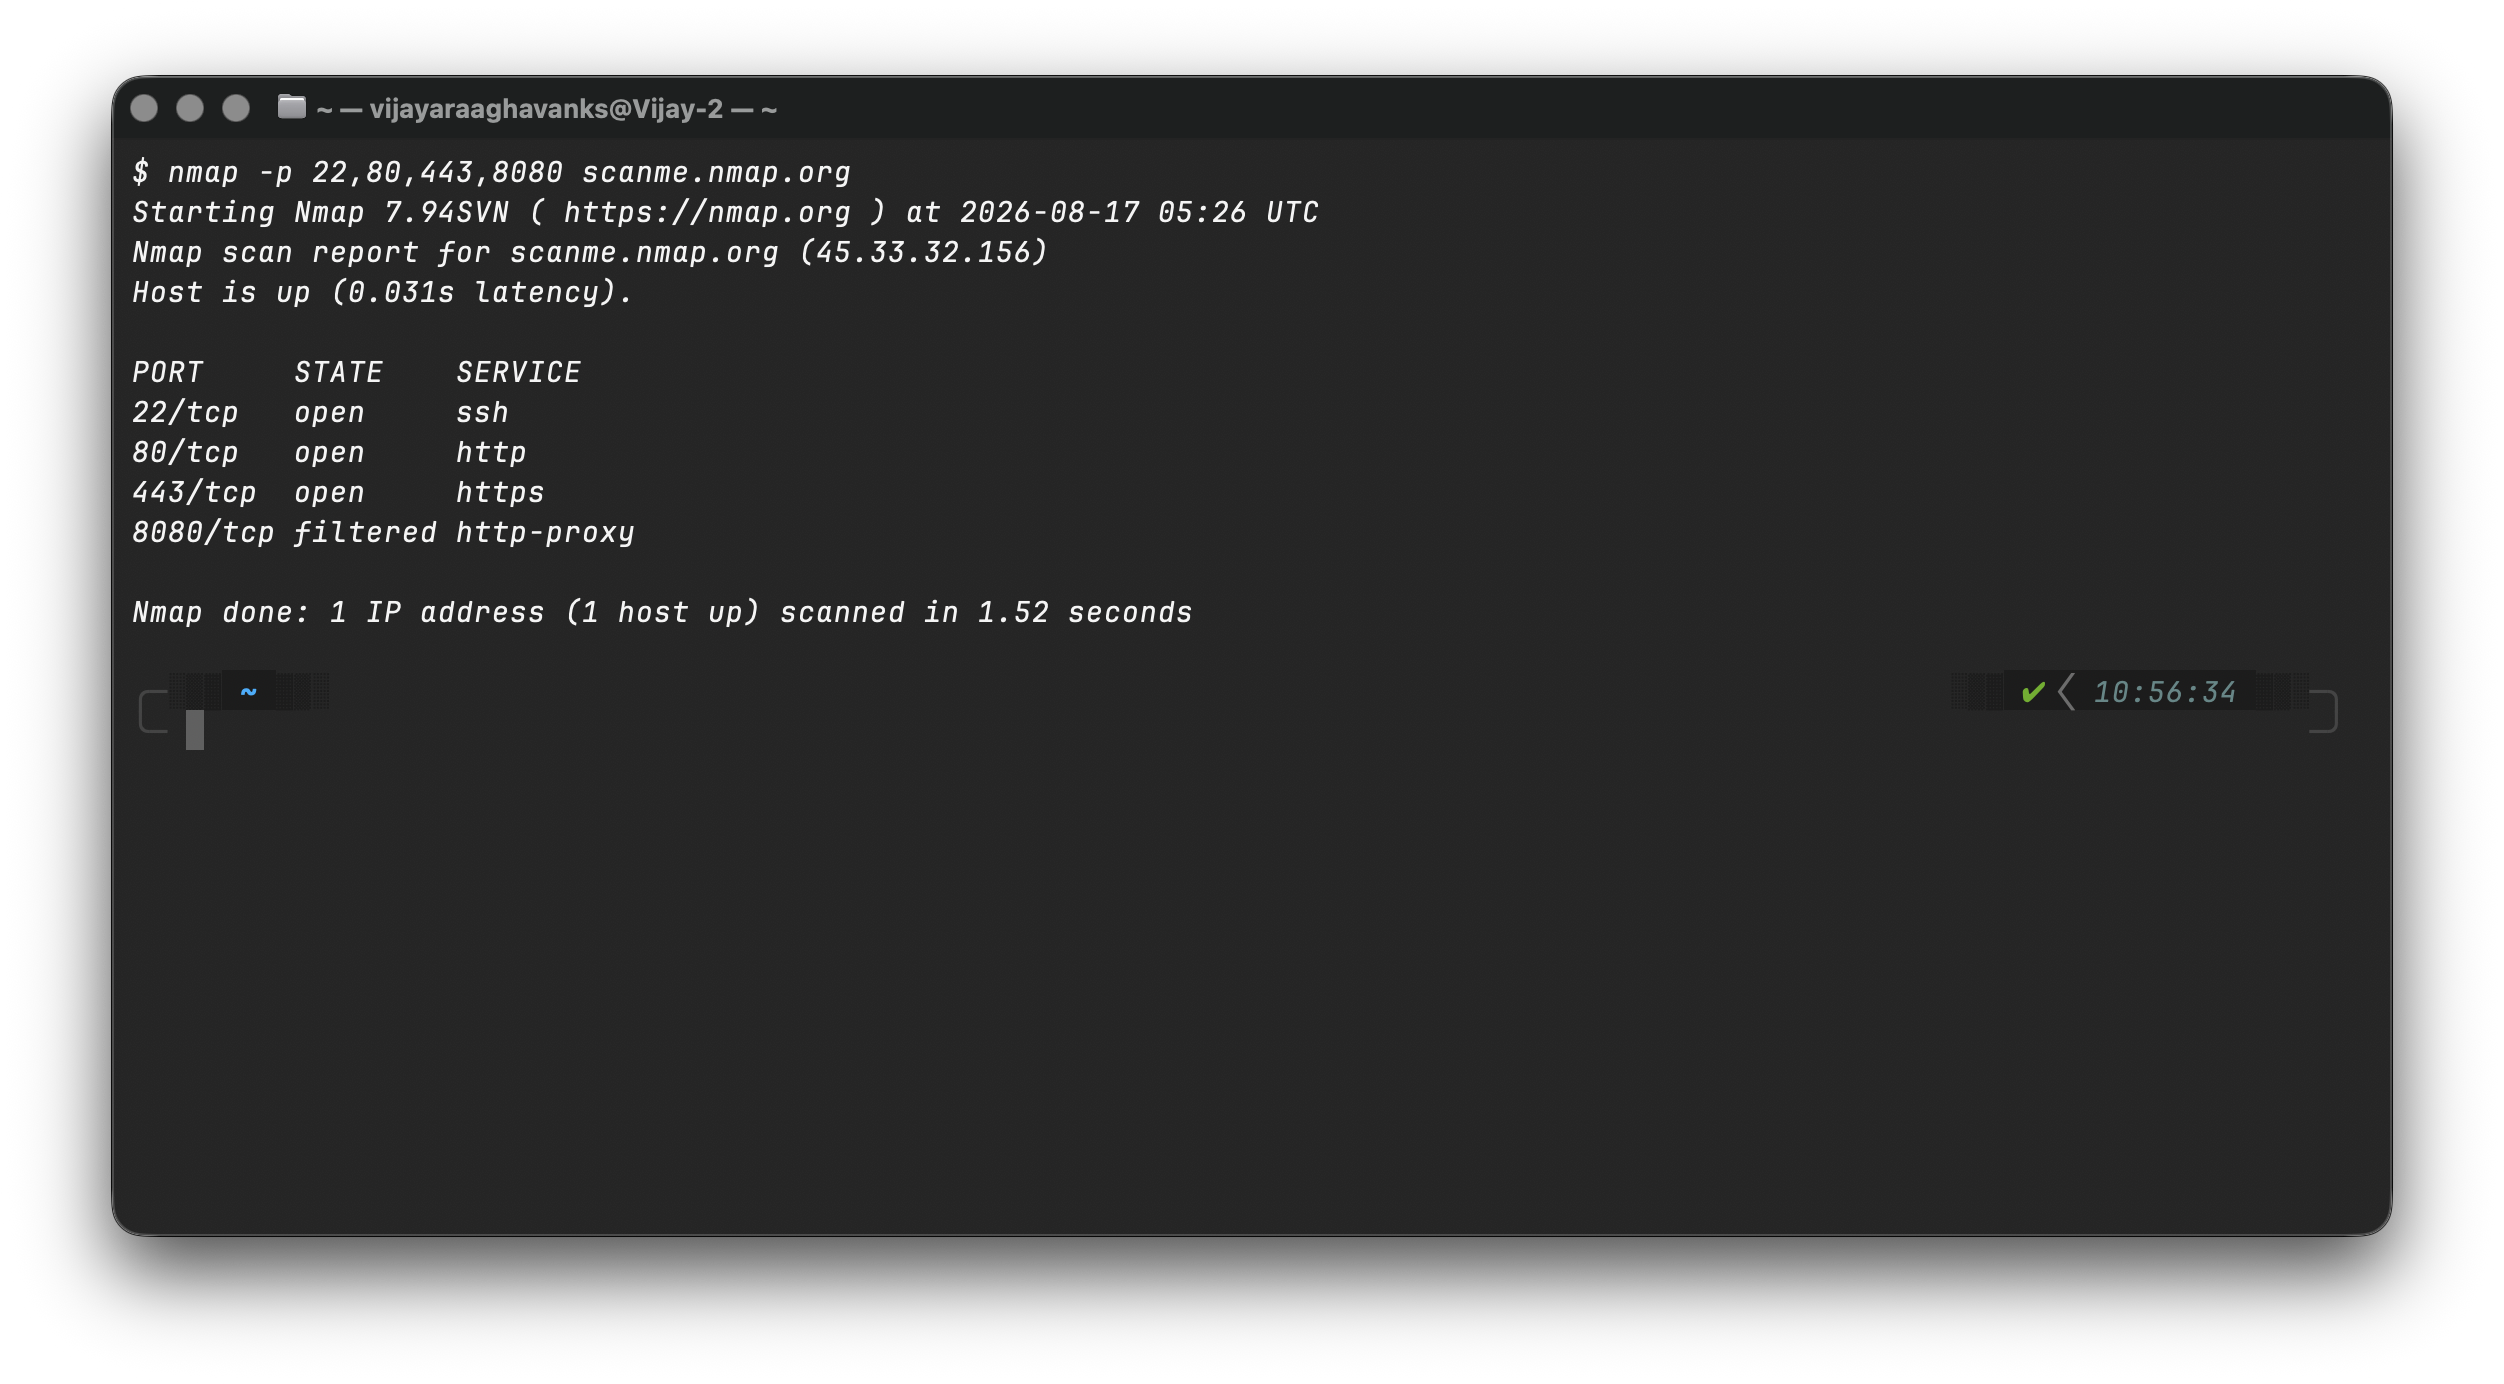
\includegraphics[width=0.8\linewidth]{screenshots/06_nmap.png}\caption{nmap port scan of scanme.nmap.org}\end{figure}

\subsection*{2.7 tcpdump -- live packet capture}
\begin{lstlisting}[style=bashstyle]
$ tcpdump -c 5 -i eth0
\end{lstlisting}
\texttt{tcpdump} captures and prints packets crossing an interface in real time. While a
background \texttt{ping} to \texttt{8.8.8.8} was running, \texttt{tcpdump} captured 5 packets on
\texttt{eth0}: ICMP echo request/reply pairs and, interestingly, a DNS PTR (reverse-lookup)
query/response pair for \texttt{8.8.8.8.in-addr.arpa} triggered automatically -- both traffic
types are visible with full source/destination and protocol detail.
\begin{figure}[h!]\centering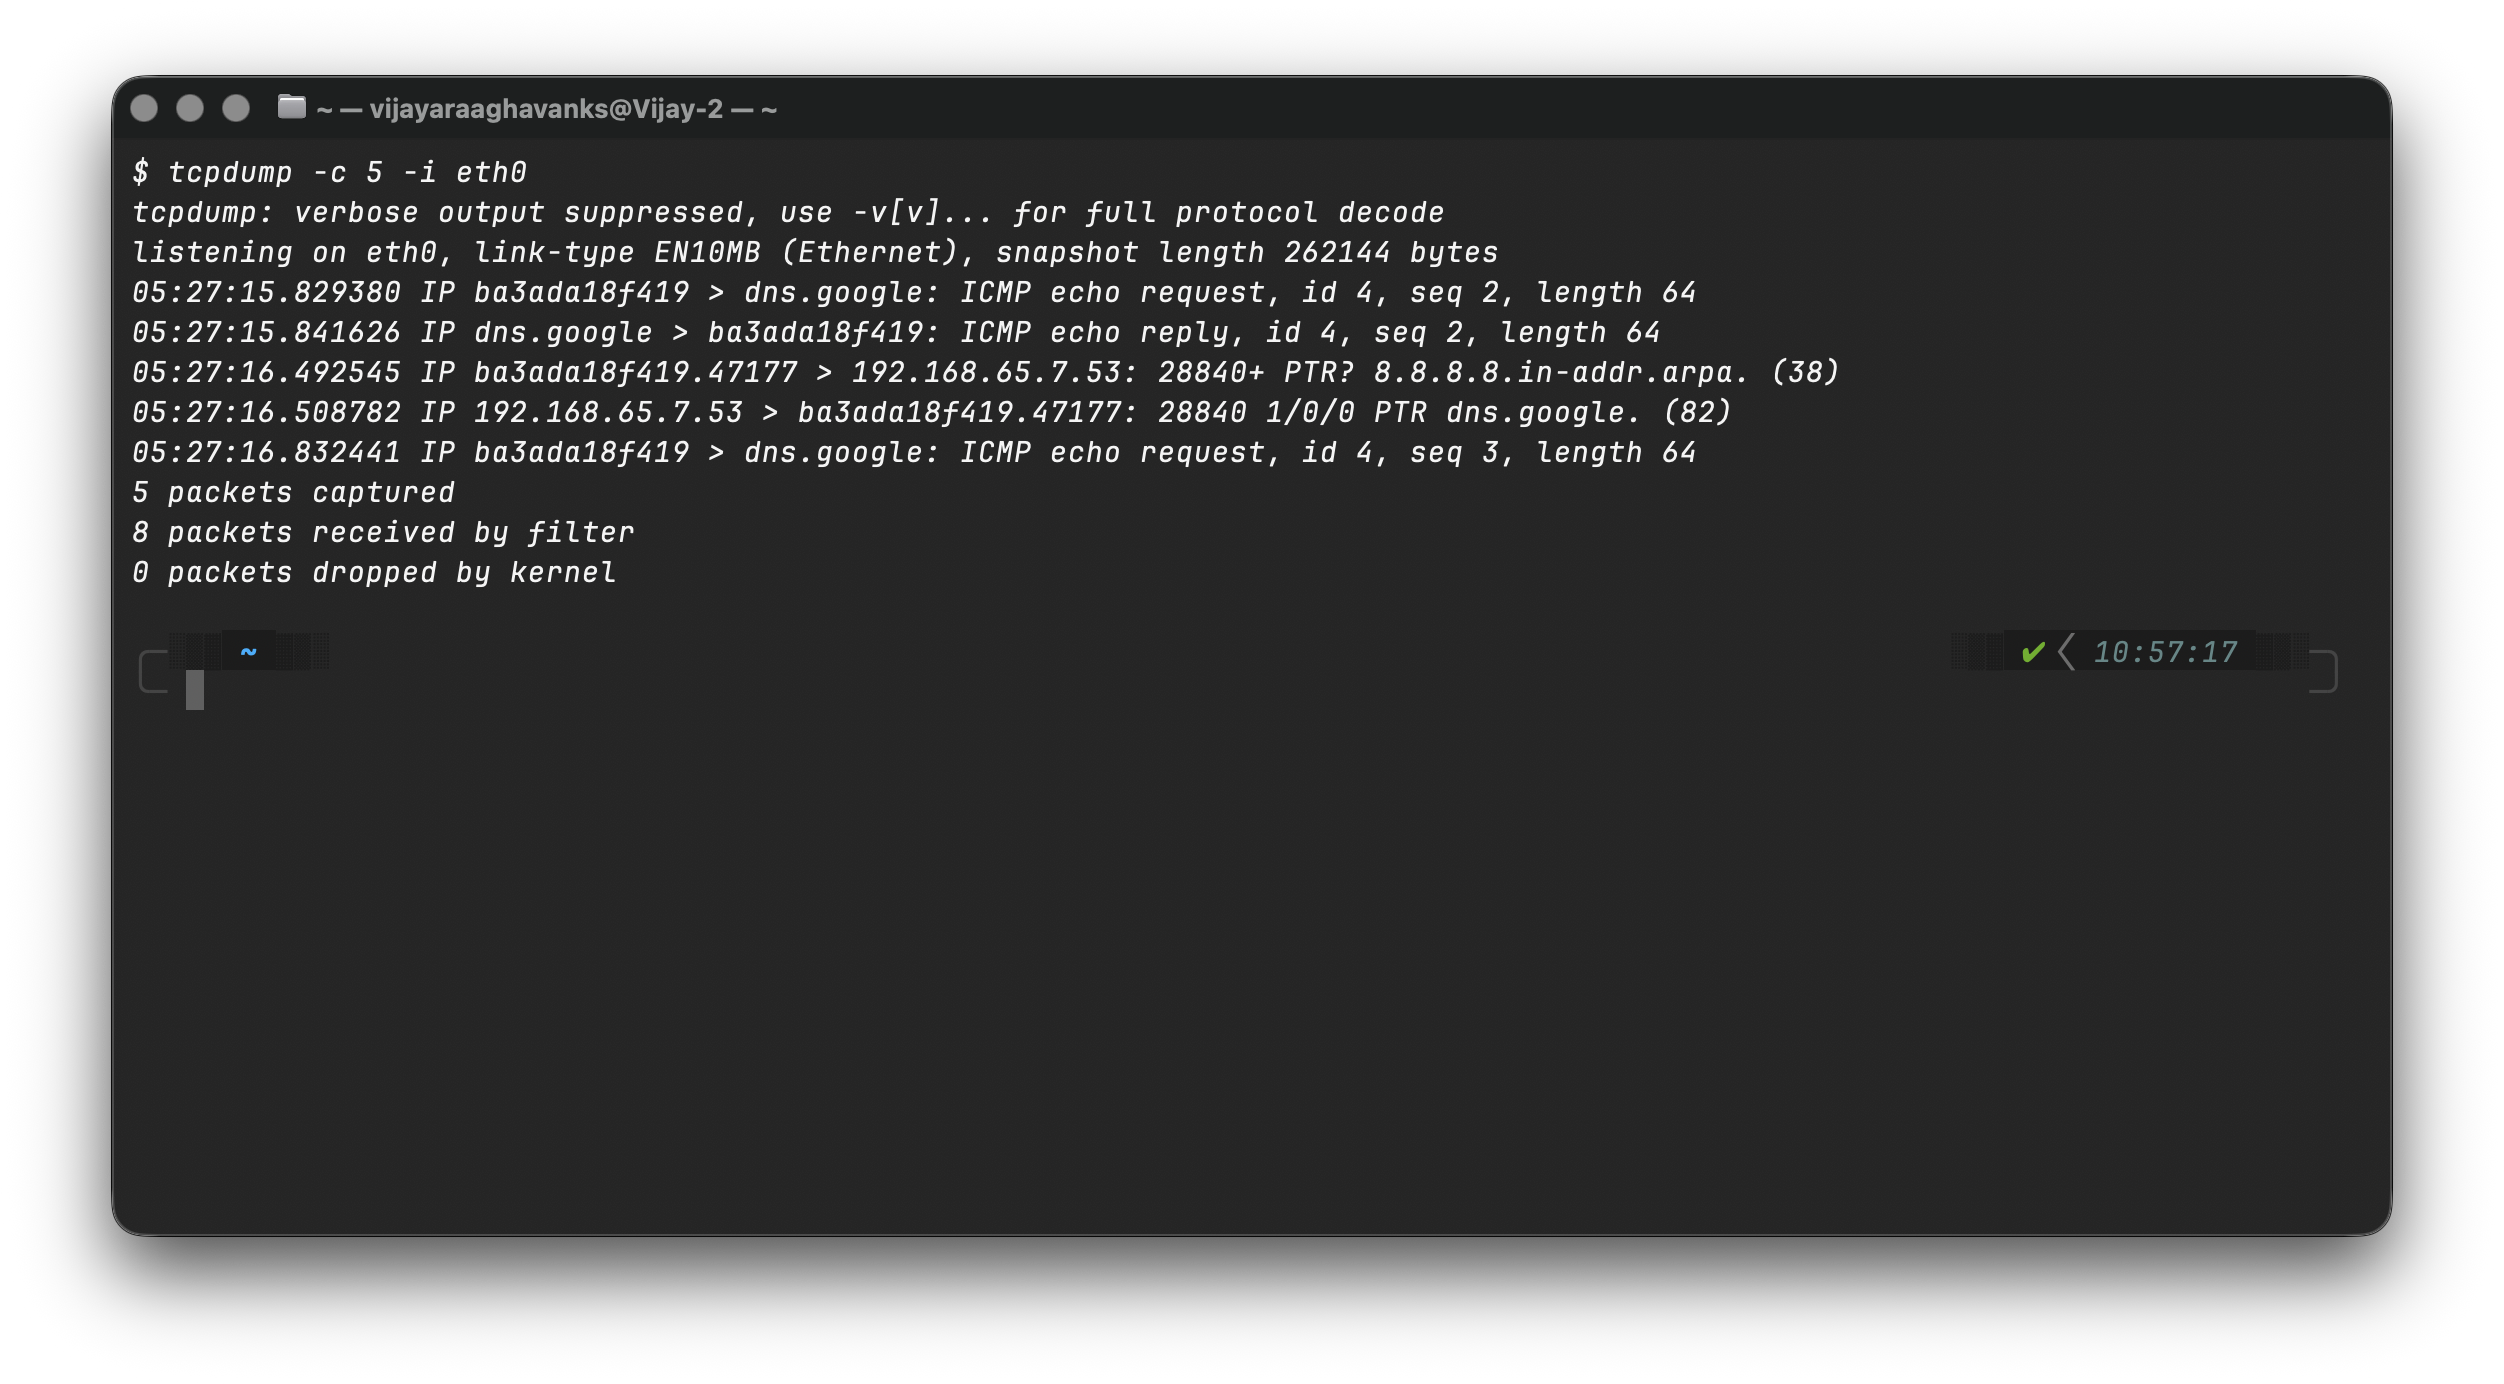
\includegraphics[width=0.8\linewidth]{screenshots/07_tcpdump.png}\caption{tcpdump -- live capture of ICMP and DNS PTR traffic}\end{figure}

\subsection*{2.8 dig -- detailed DNS query}
\begin{lstlisting}[style=bashstyle]
$ dig google.com
\end{lstlisting}
\texttt{dig} performs a DNS lookup and prints the full query/response structure. The
\texttt{ANSWER SECTION} shows an \texttt{A} record for \texttt{google.com} resolving to
\texttt{142.250.206.78} with TTL 350\,s, answered by the resolver \texttt{192.168.65.7} in
2\,ms over UDP.
\begin{figure}[h!]\centering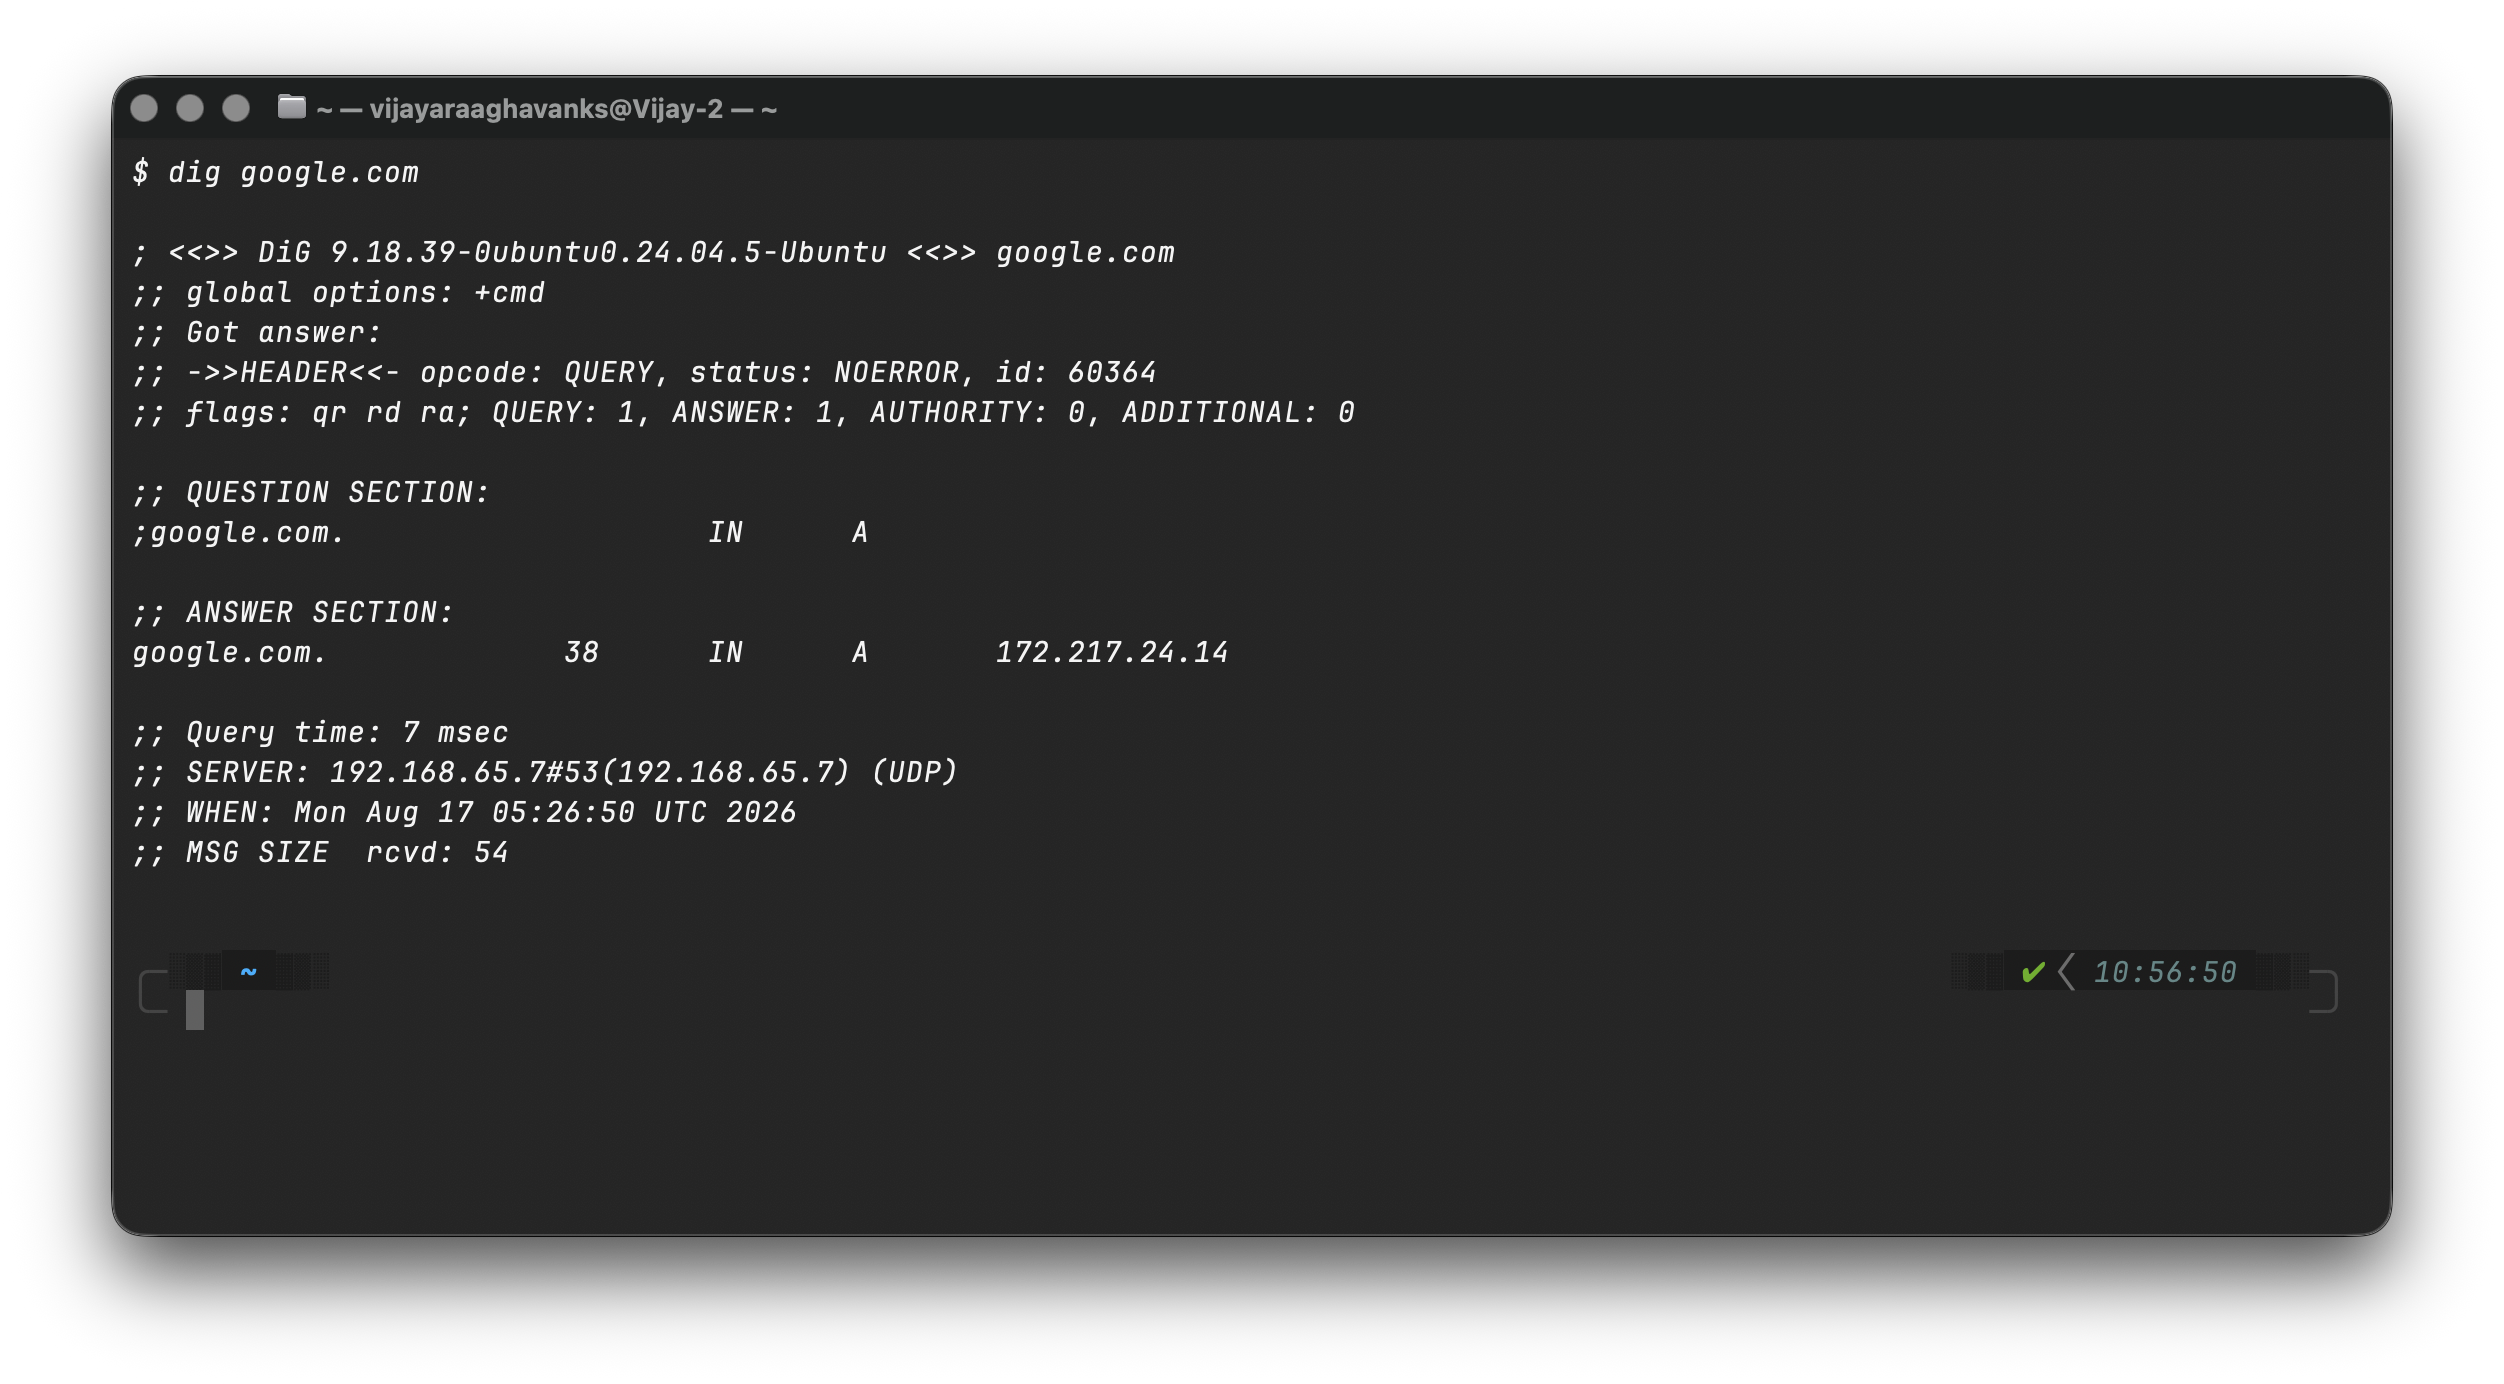
\includegraphics[width=0.8\linewidth]{screenshots/08_dig.png}\caption{dig google.com -- full DNS answer section}\end{figure}

\subsection*{2.9 traceroute -- hop-by-hop path discovery}
\begin{lstlisting}[style=bashstyle]
$ traceroute -w 1 -q 1 -m 10 google.com
\end{lstlisting}
\texttt{traceroute} discovers the path to a destination by sending probes with increasing TTL
and recording which router returns an ICMP Time-Exceeded message at each hop. Only hop 1 (the
Docker gateway \texttt{172.17.0.1}) replied; hops 2--10 show \texttt{*}, since Docker Desktop's
NAT layer does not generate or forward ICMP Time-Exceeded messages for the intermediate hops
back into the container -- the packets do reach Google (confirmed by \texttt{ping}/\texttt{dig}
above) but the diagnostic ICMP replies used by traceroute are filtered.
\begin{figure}[h!]\centering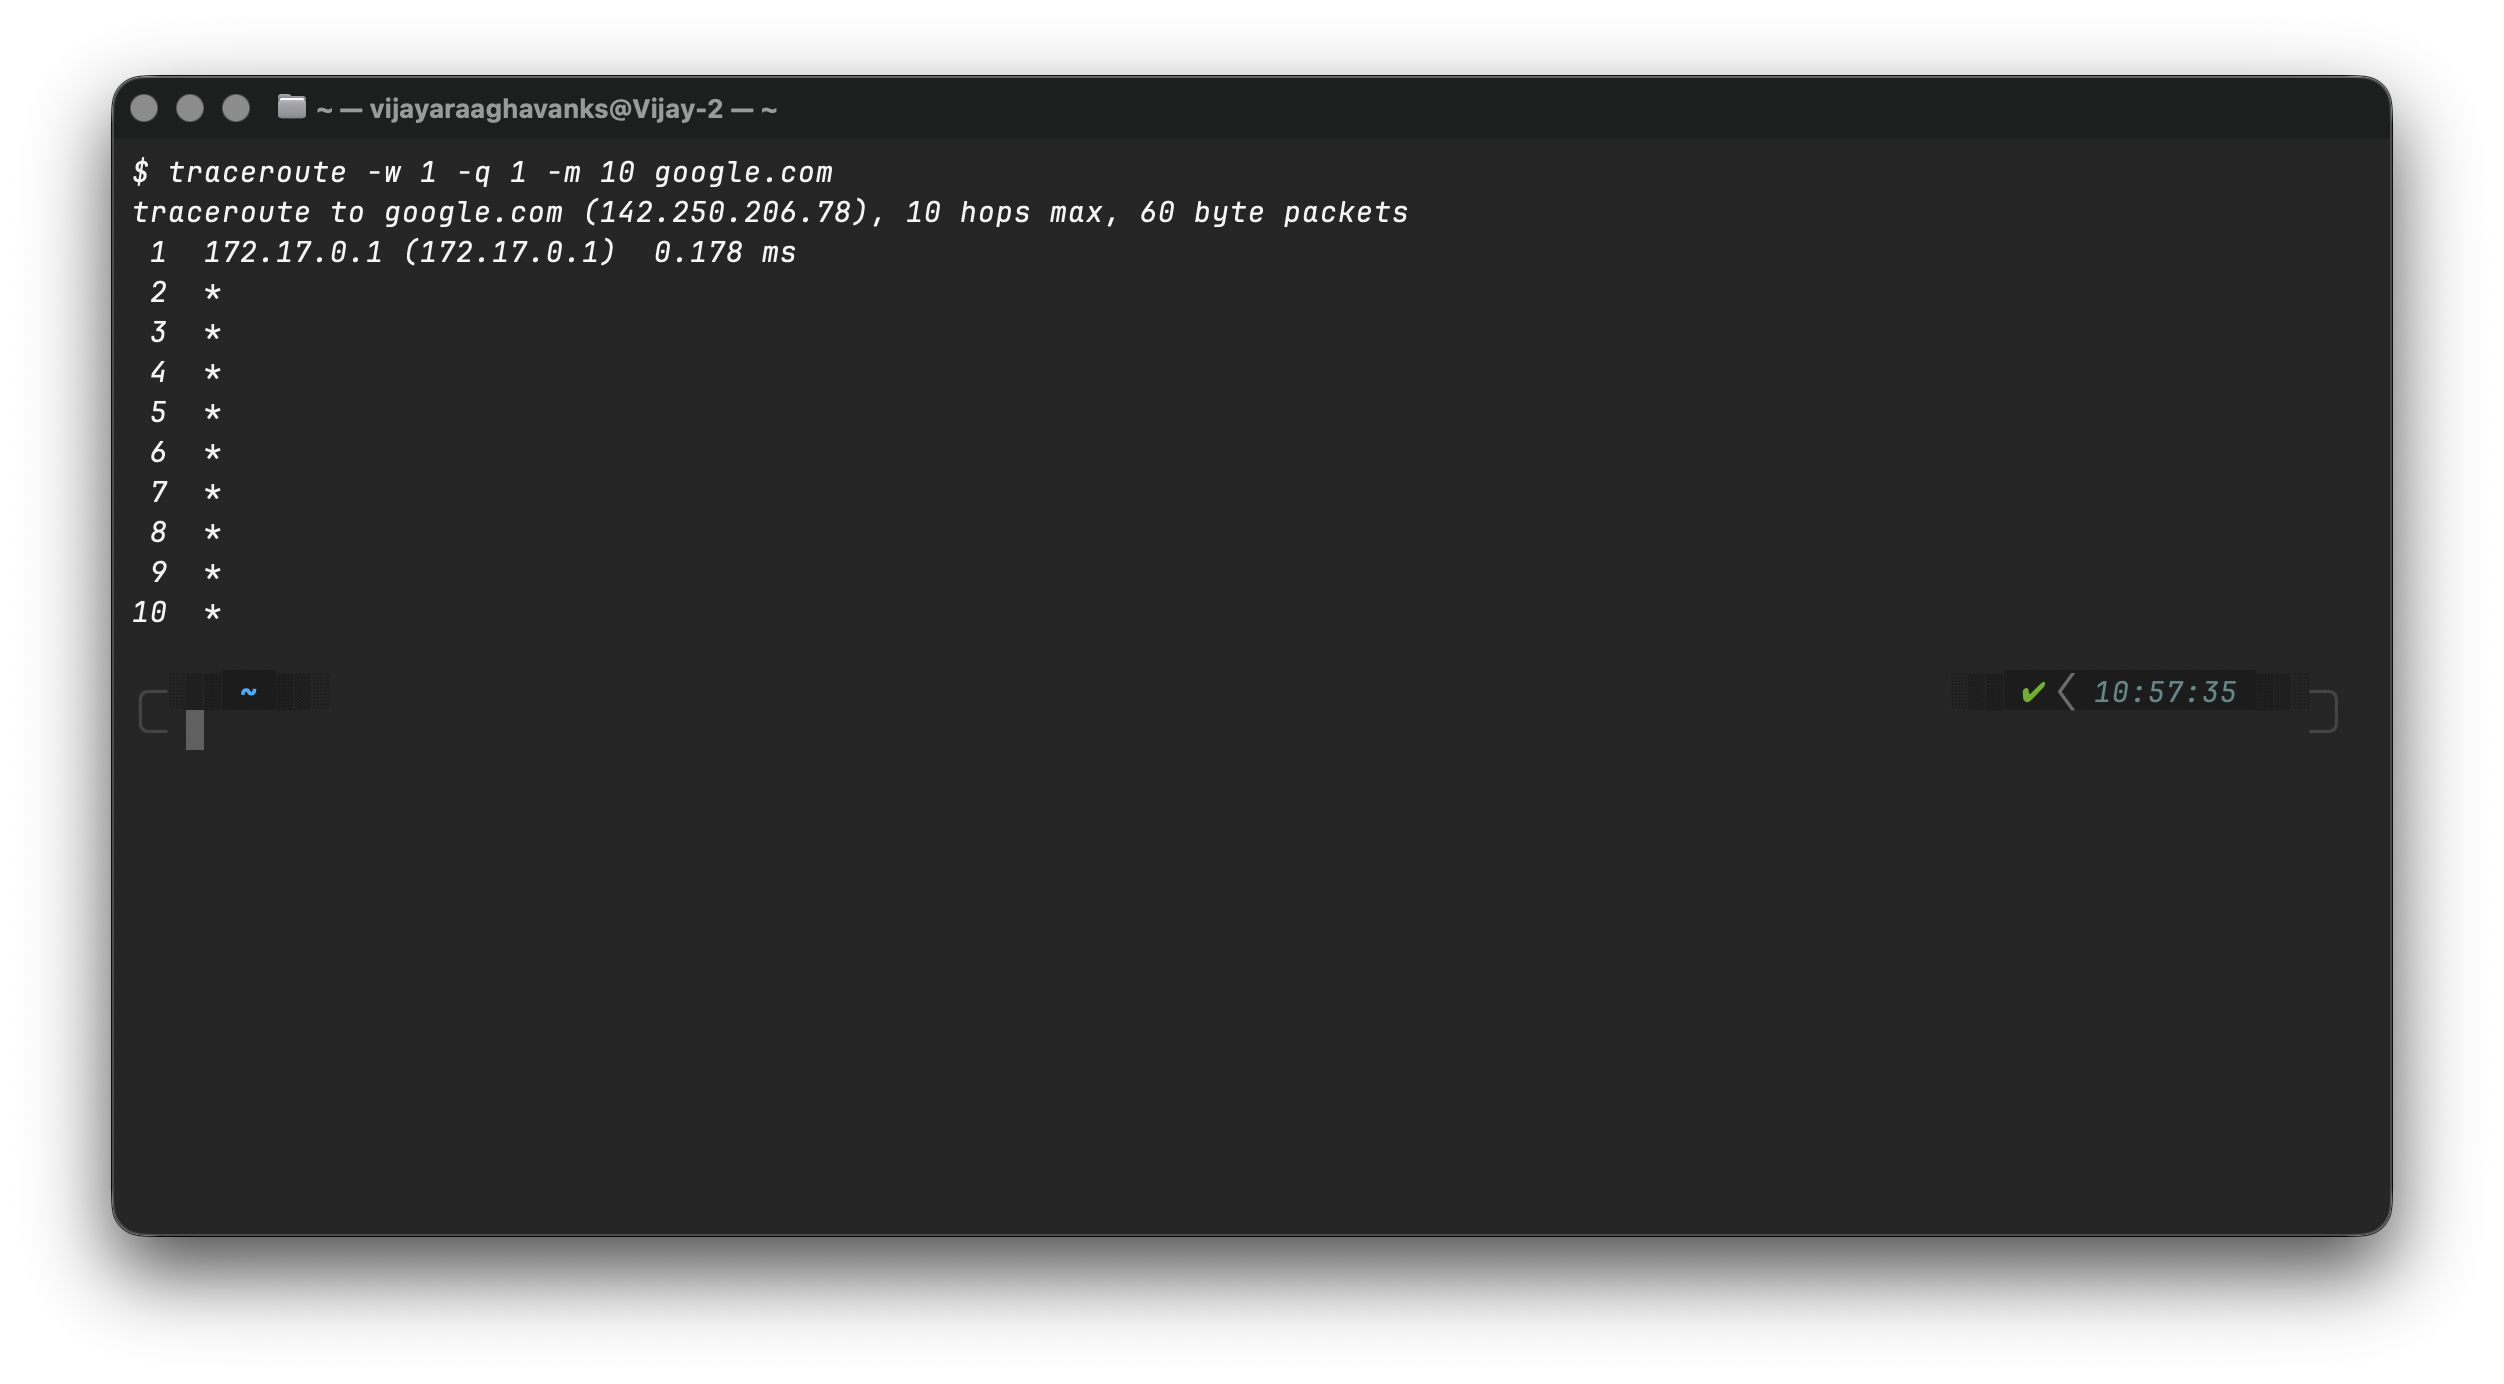
\includegraphics[width=0.8\linewidth]{screenshots/09_traceroute.png}\caption{traceroute to google.com -- only the local gateway hop responds}\end{figure}

\subsection*{2.10 mtr -- continuous traceroute + ping}
\begin{lstlisting}[style=bashstyle]
$ mtr -c 3 --report -n google.com
\end{lstlisting}
\texttt{mtr} combines \texttt{ping} and \texttt{traceroute}, sending repeated probes to every
hop and reporting live loss/latency statistics. Unlike \texttt{traceroute}, \texttt{mtr}'s
report shows only \textbf{two} hops -- the gateway (\texttt{172.17.0.1}, 0\% loss,
avg 0.1\,ms) and \texttt{google.com} itself (\texttt{142.250.206.78}, 0\% loss, avg 12.8\,ms)
-- because \texttt{mtr} silently skips non-responding intermediate hops in its summary table
rather than printing \texttt{*} placeholders.
\begin{figure}[h!]\centering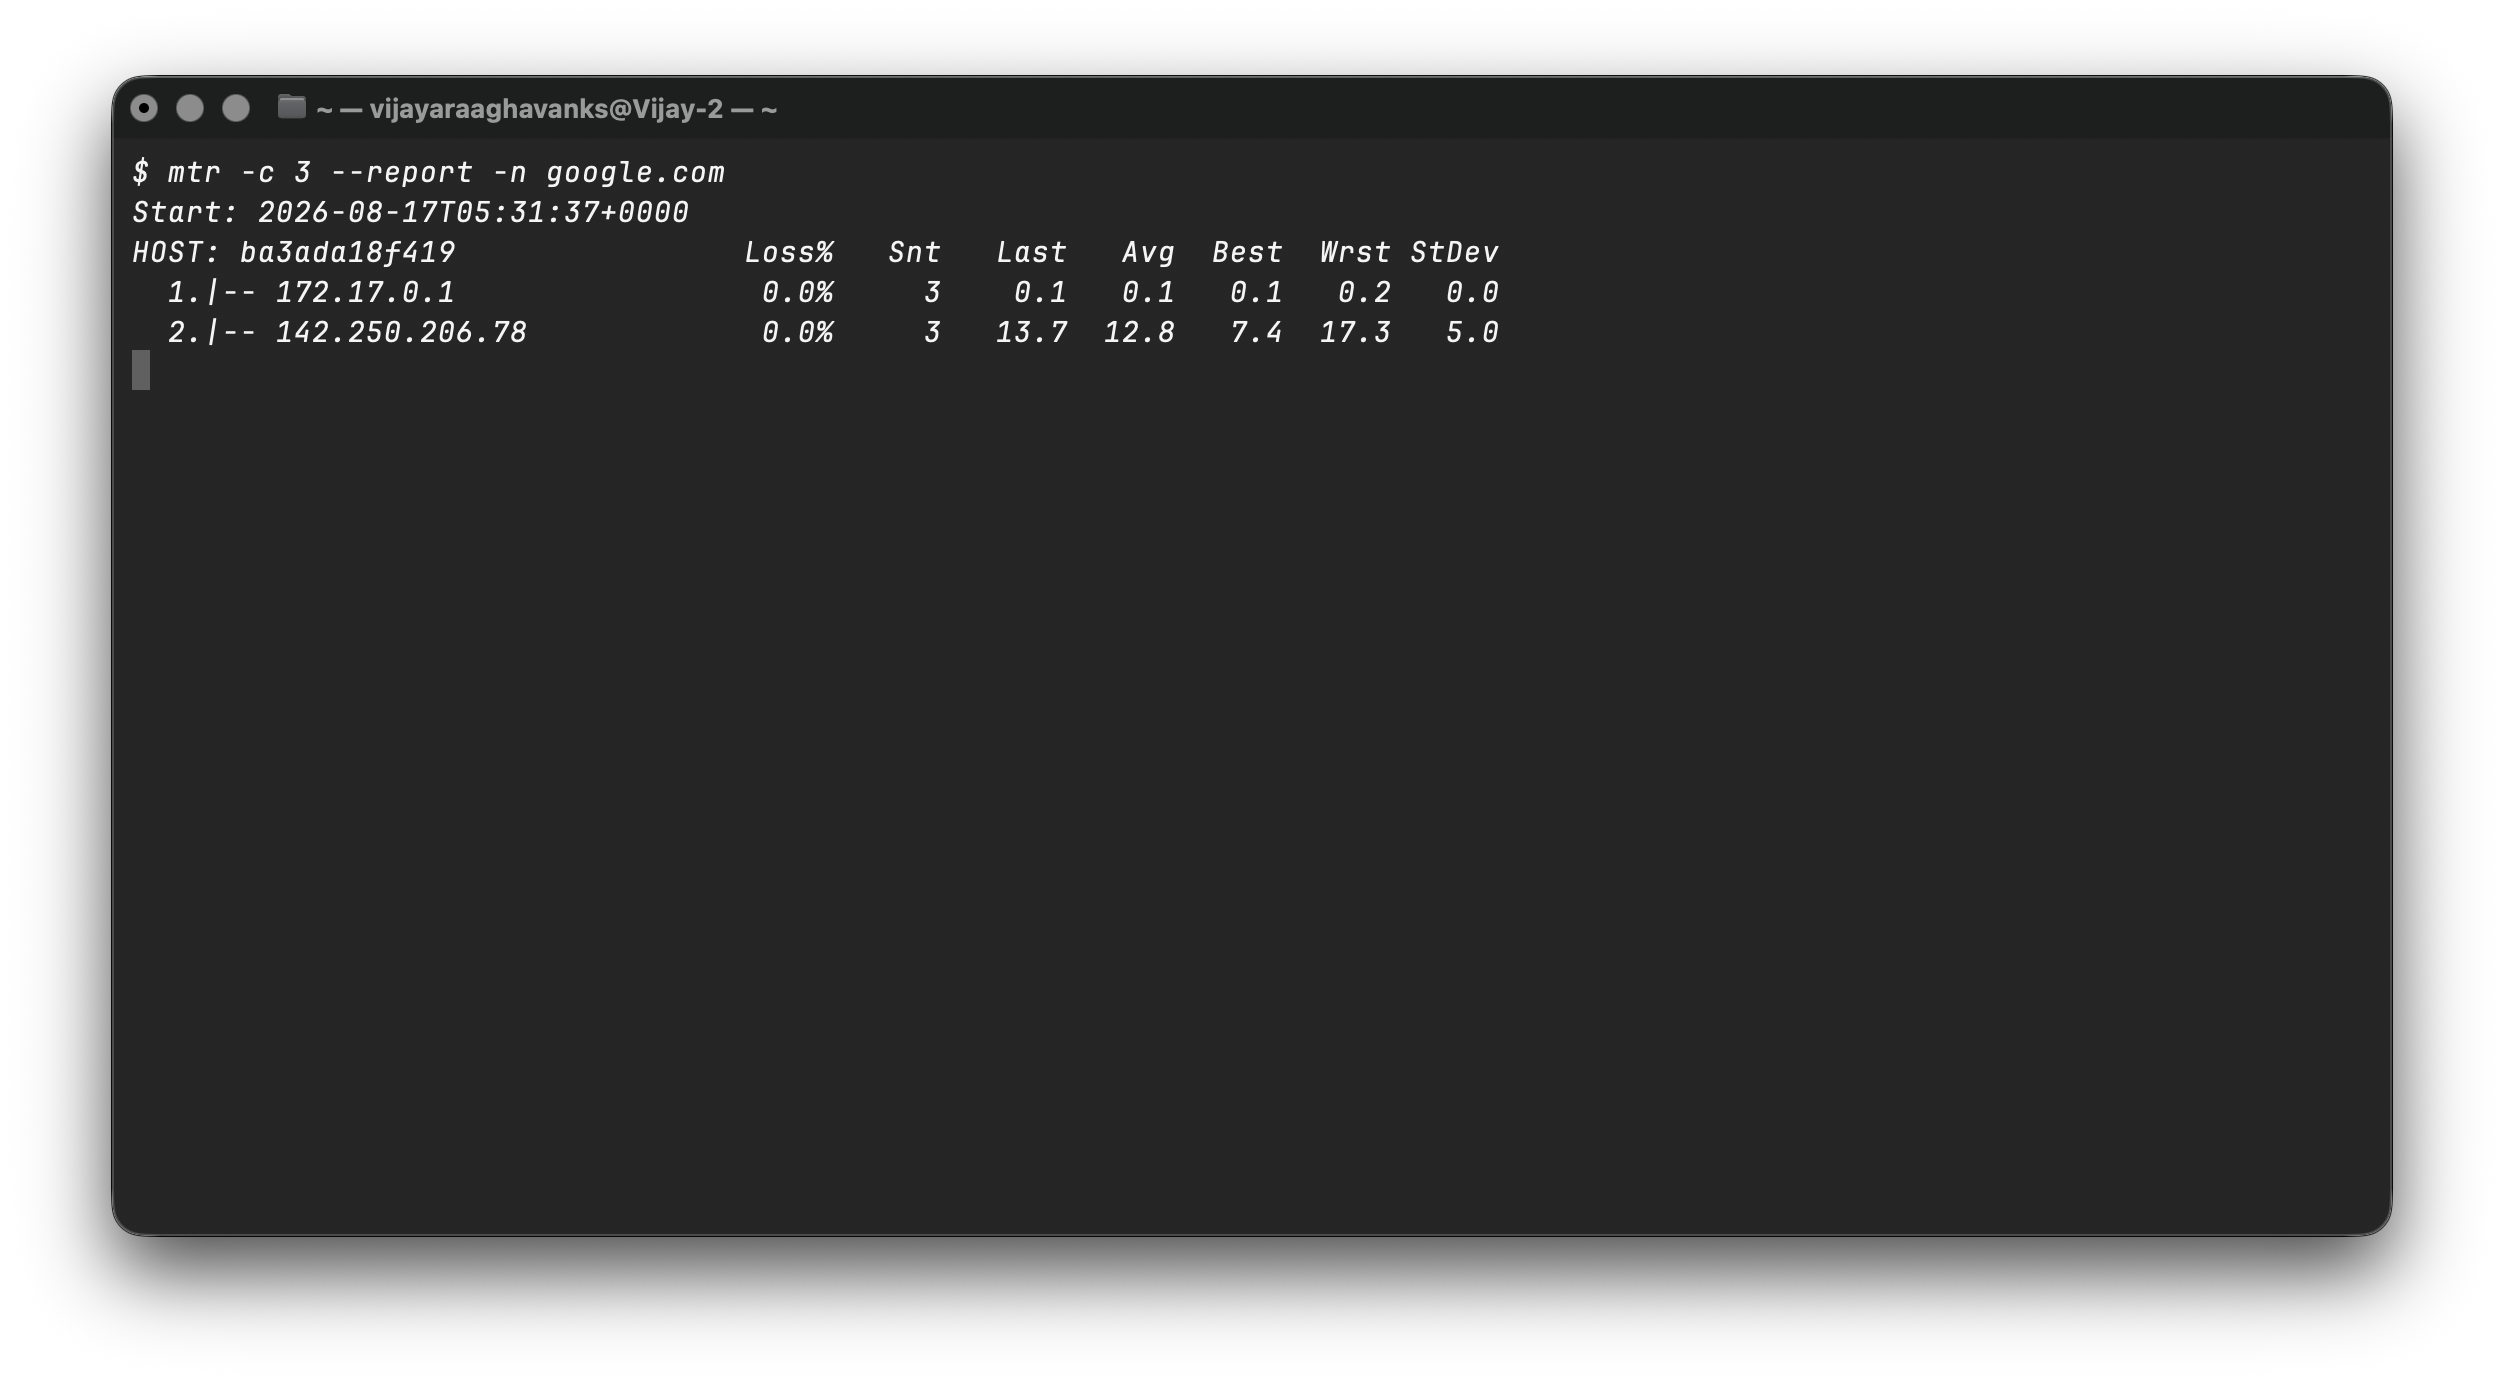
\includegraphics[width=0.8\linewidth]{screenshots/10_mtr.png}\caption{mtr report -- gateway and destination statistics}\end{figure}

\subsection*{2.11 curl -- HTTP request from the command line}
\begin{lstlisting}[style=bashstyle]
$ curl -I https://www.google.com
\end{lstlisting}
\texttt{curl -I} sends an HTTP \texttt{HEAD} request and prints only the response headers.
Google responded \texttt{HTTP/2 200}, and the header block reveals the content type, CSP
policy, \texttt{Set-Cookie} values, and \texttt{Alt-Svc} advertisement of HTTP/3 (QUIC)
support.
\begin{figure}[h!]\centering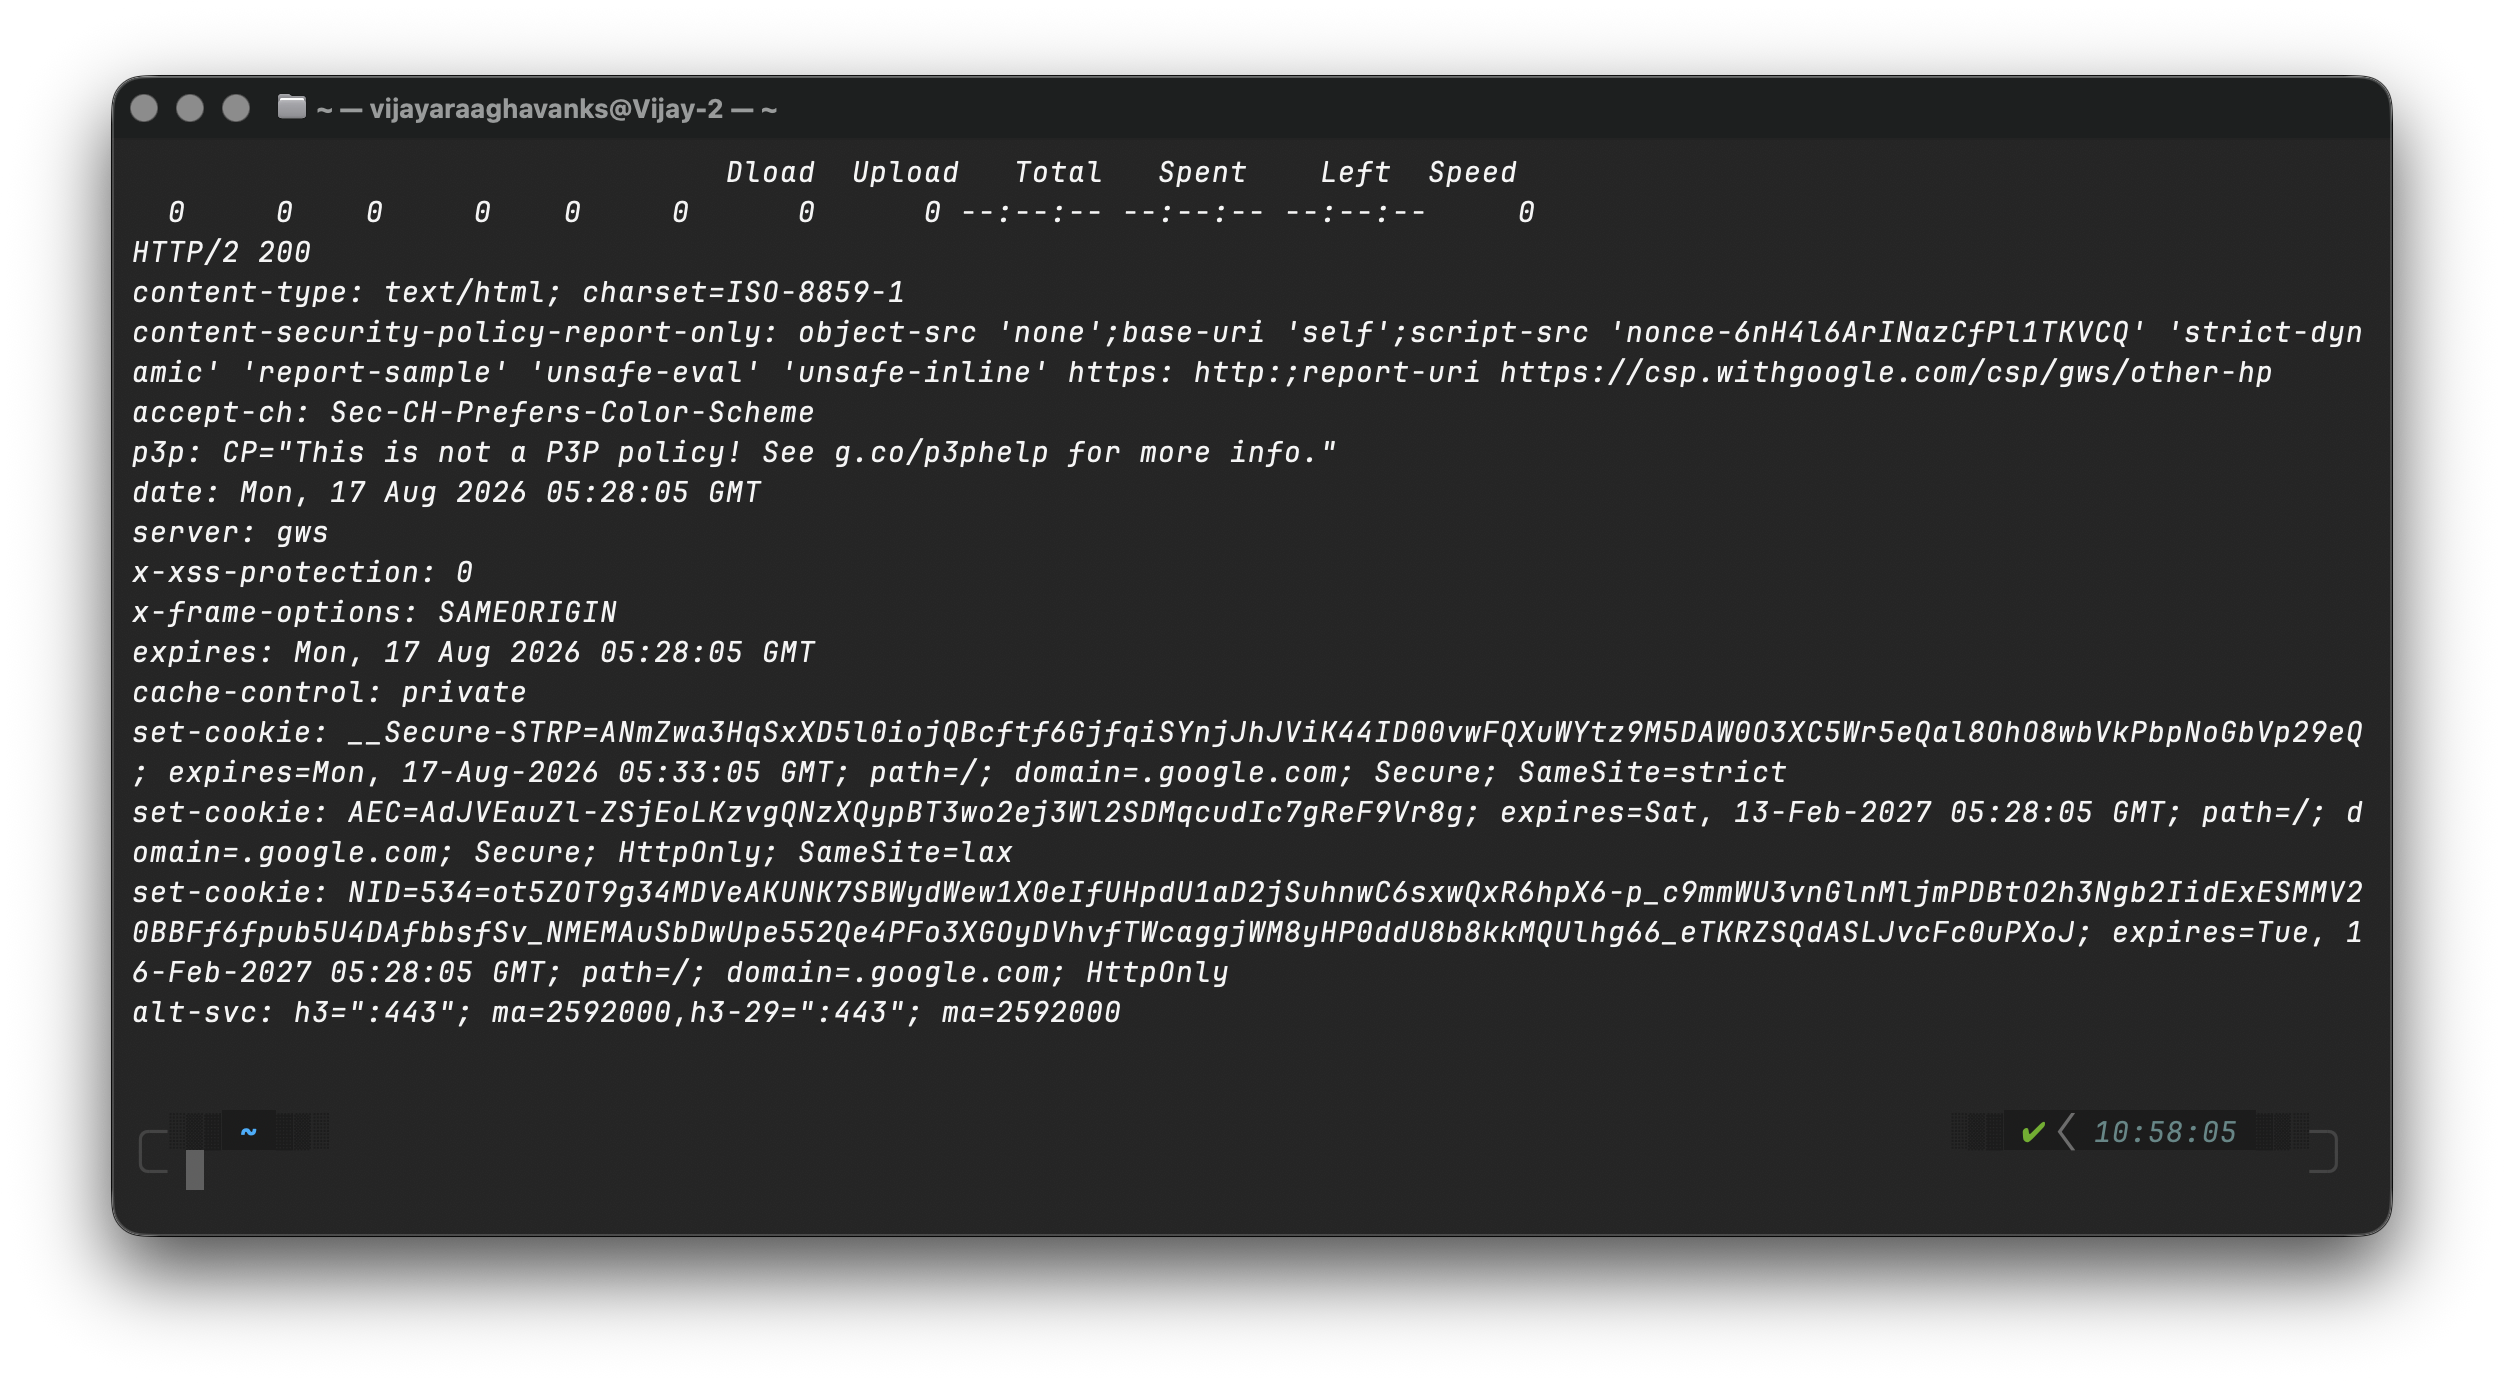
\includegraphics[width=0.8\linewidth]{screenshots/11_curl.png}\caption{curl -I https://www.google.com -- HTTP/2 200 response headers}\end{figure}

\subsection*{2.12 wget -- HTTP request / download client}
\begin{lstlisting}[style=bashstyle]
$ wget -S --spider https://www.google.com
\end{lstlisting}
\texttt{wget --spider} checks whether a resource exists without downloading it, while
\texttt{-S} prints the server response headers. The output shows the DNS resolution of
\texttt{www.google.com} to multiple A records, a successful TLS connection on port 443, and an
\texttt{HTTP/1.1 200 OK} response -- confirming the resource is reachable.
\begin{figure}[h!]\centering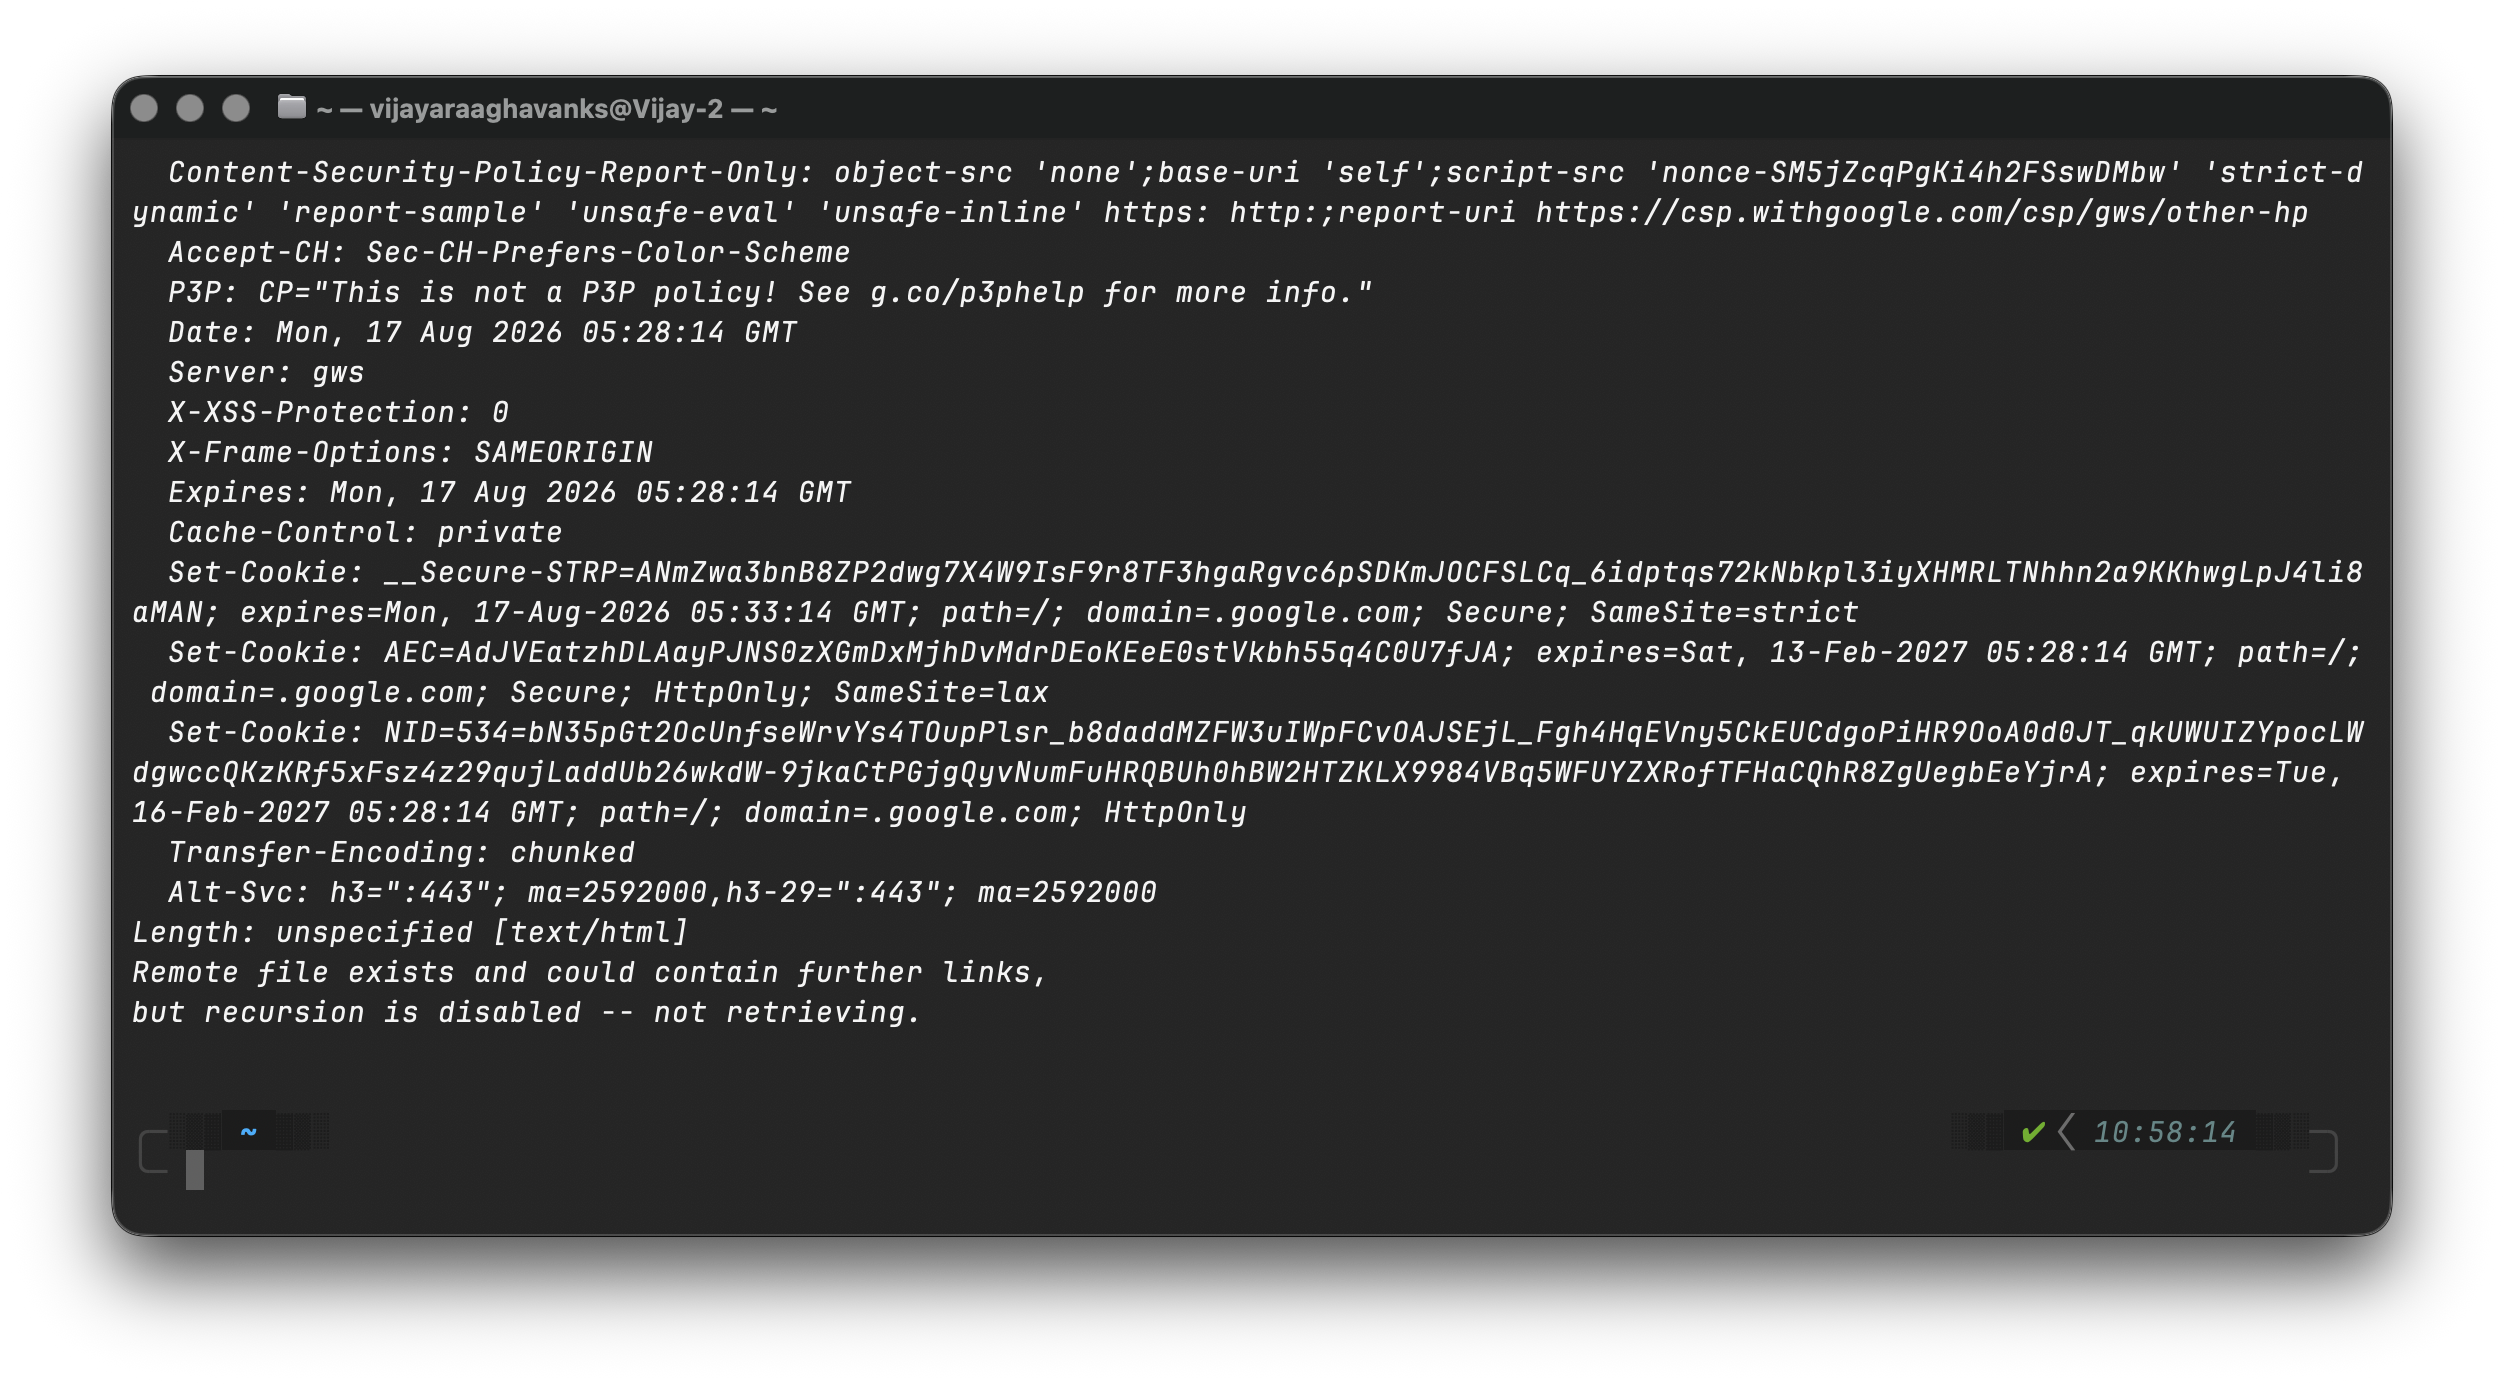
\includegraphics[width=0.8\linewidth]{screenshots/12_wget.png}\caption{wget --spider -S -- resolving, connecting and header dump}\end{figure}

\subsection*{2.13 tracepath -- unprivileged path MTU discovery}
\begin{lstlisting}[style=bashstyle]
$ tracepath -m 8 google.com
\end{lstlisting}
\texttt{tracepath} is a traceroute-like tool that does not require root privileges and also
discovers the path MTU. As with \texttt{traceroute}, only hop 1 (\texttt{172.17.0.1}) responds
within the Docker NAT environment; hops 2--8 report \texttt{no reply}, and the tool reports the
default path MTU of 65535 (the container's virtual Ethernet MTU) since no smaller-MTU hop was
discovered.
\begin{figure}[h!]\centering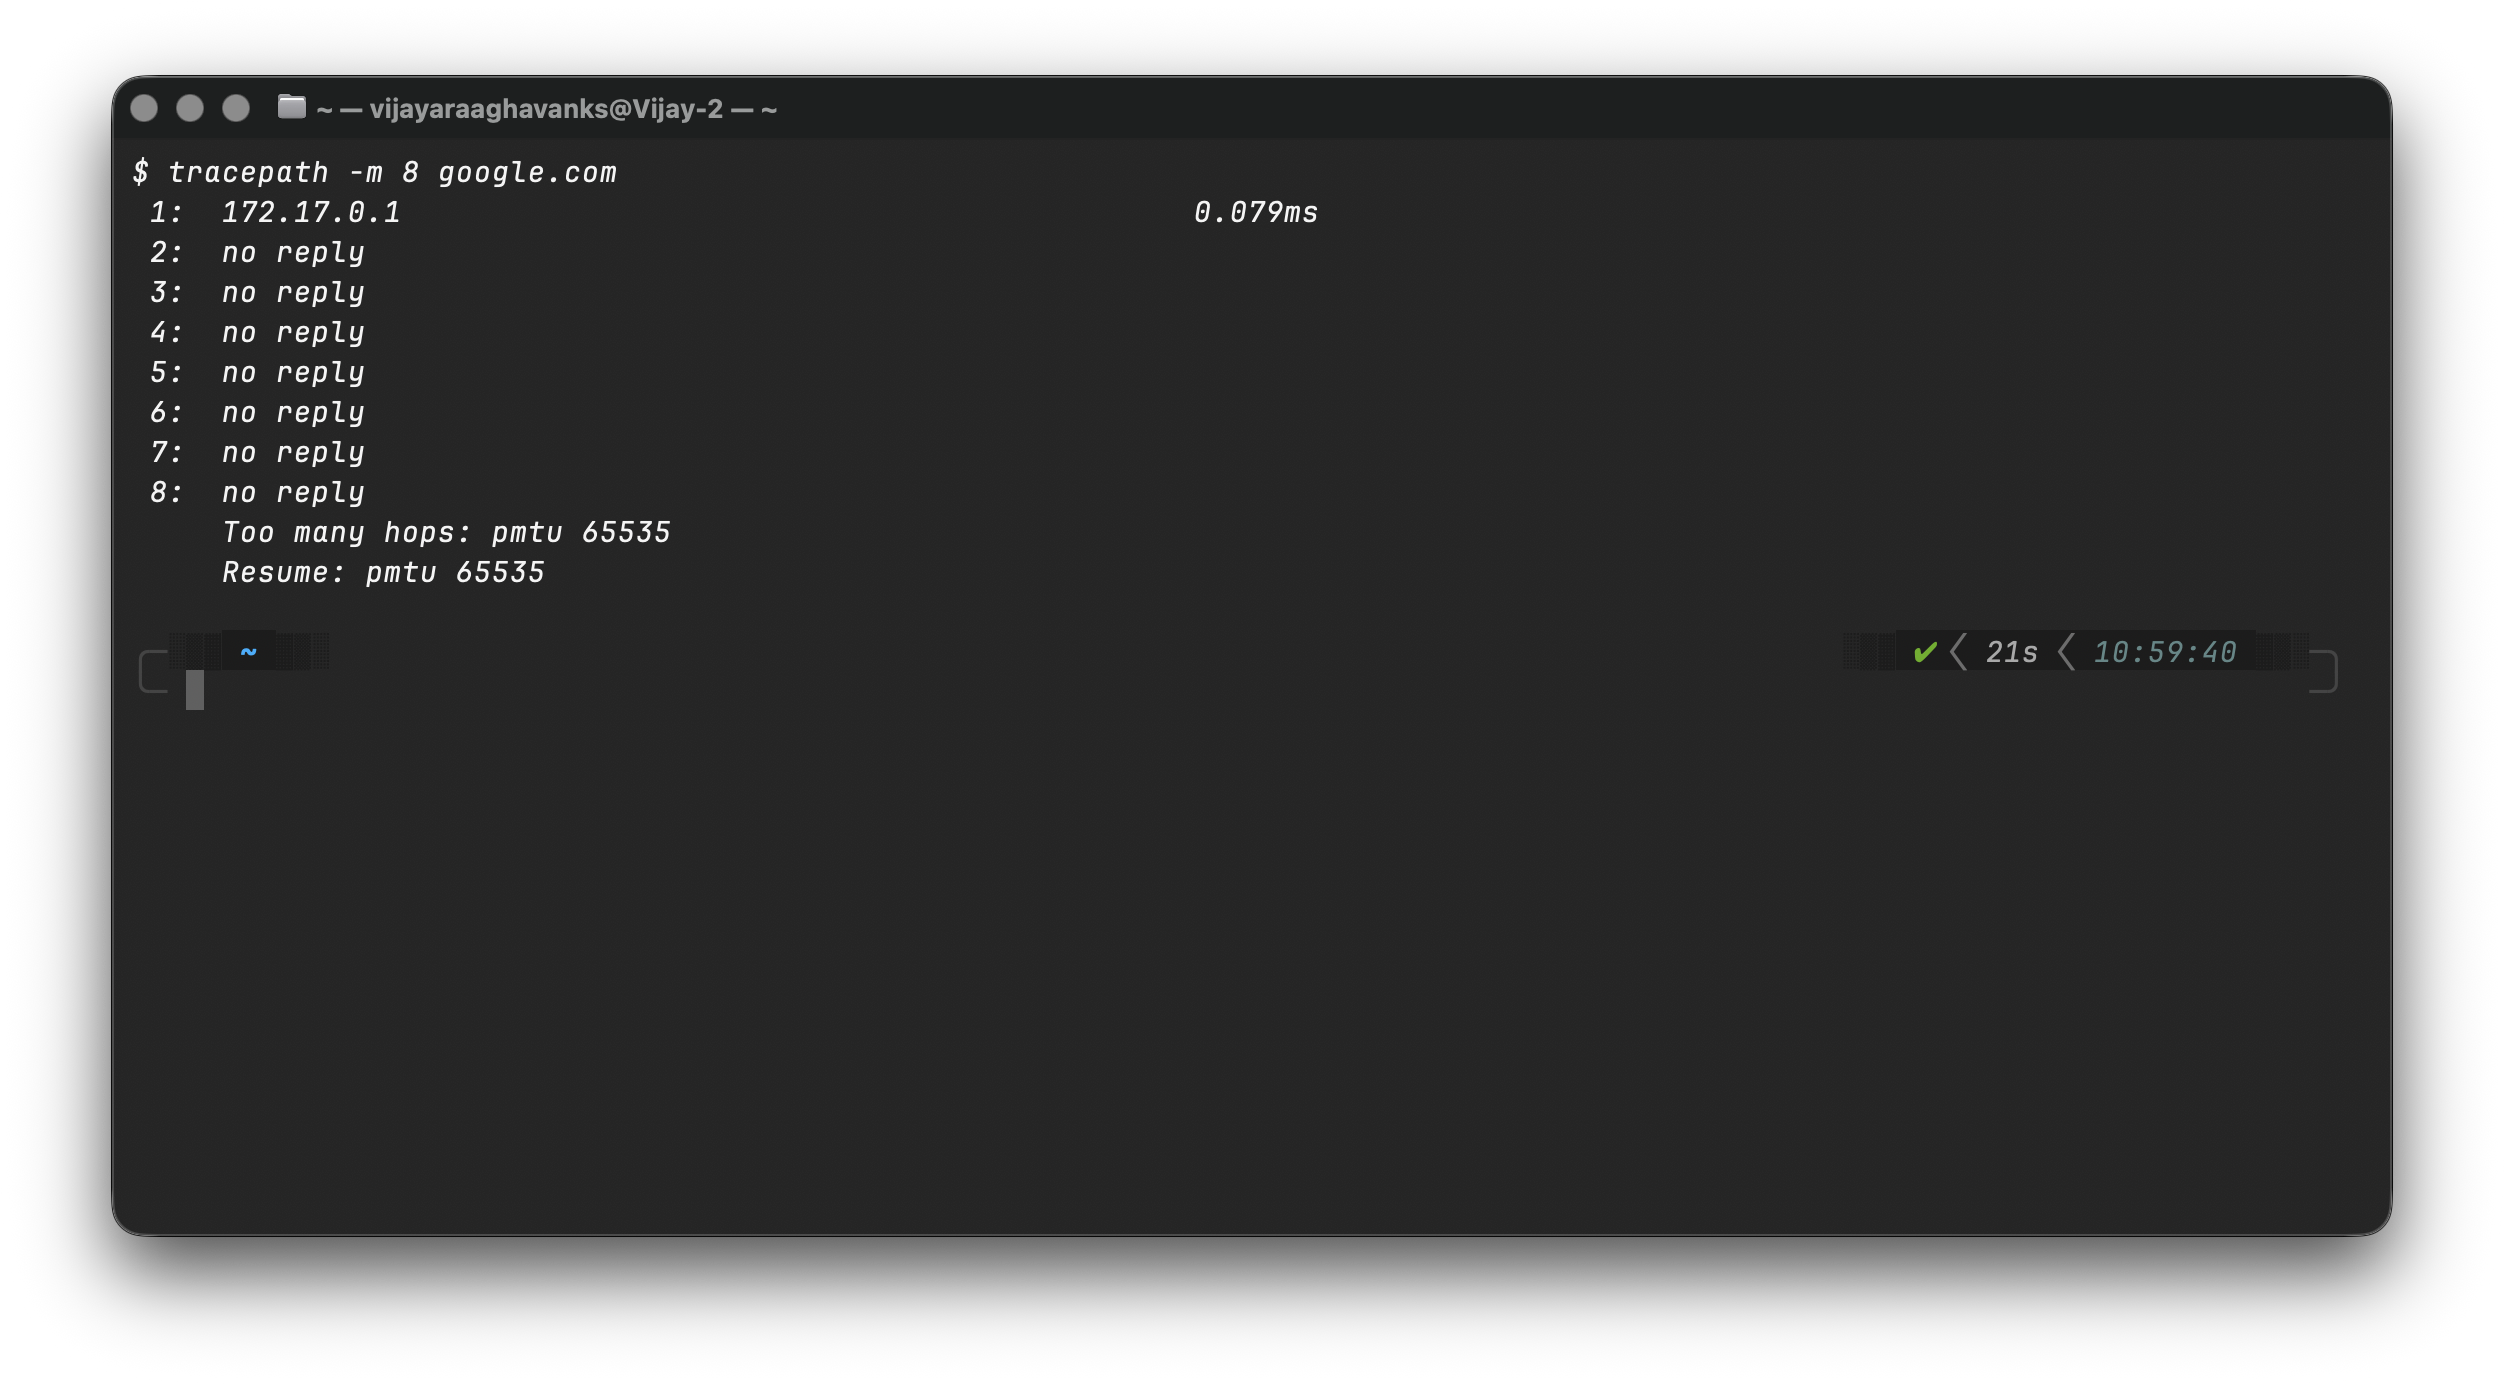
\includegraphics[width=0.8\linewidth]{screenshots/13_tracepath.png}\caption{tracepath -m 8 google.com}\end{figure}

\subsection*{2.14 nslookup -- interactive-style DNS lookup}
\begin{lstlisting}[style=bashstyle]
$ nslookup google.com
\end{lstlisting}
\texttt{nslookup} queries the configured DNS server and prints a concise answer.
\texttt{google.com} resolved (non-authoritatively, i.e.\ via a caching resolver rather than the
zone's authoritative server) to \texttt{142.250.206.78} through server \texttt{192.168.65.7}.
\begin{figure}[h!]\centering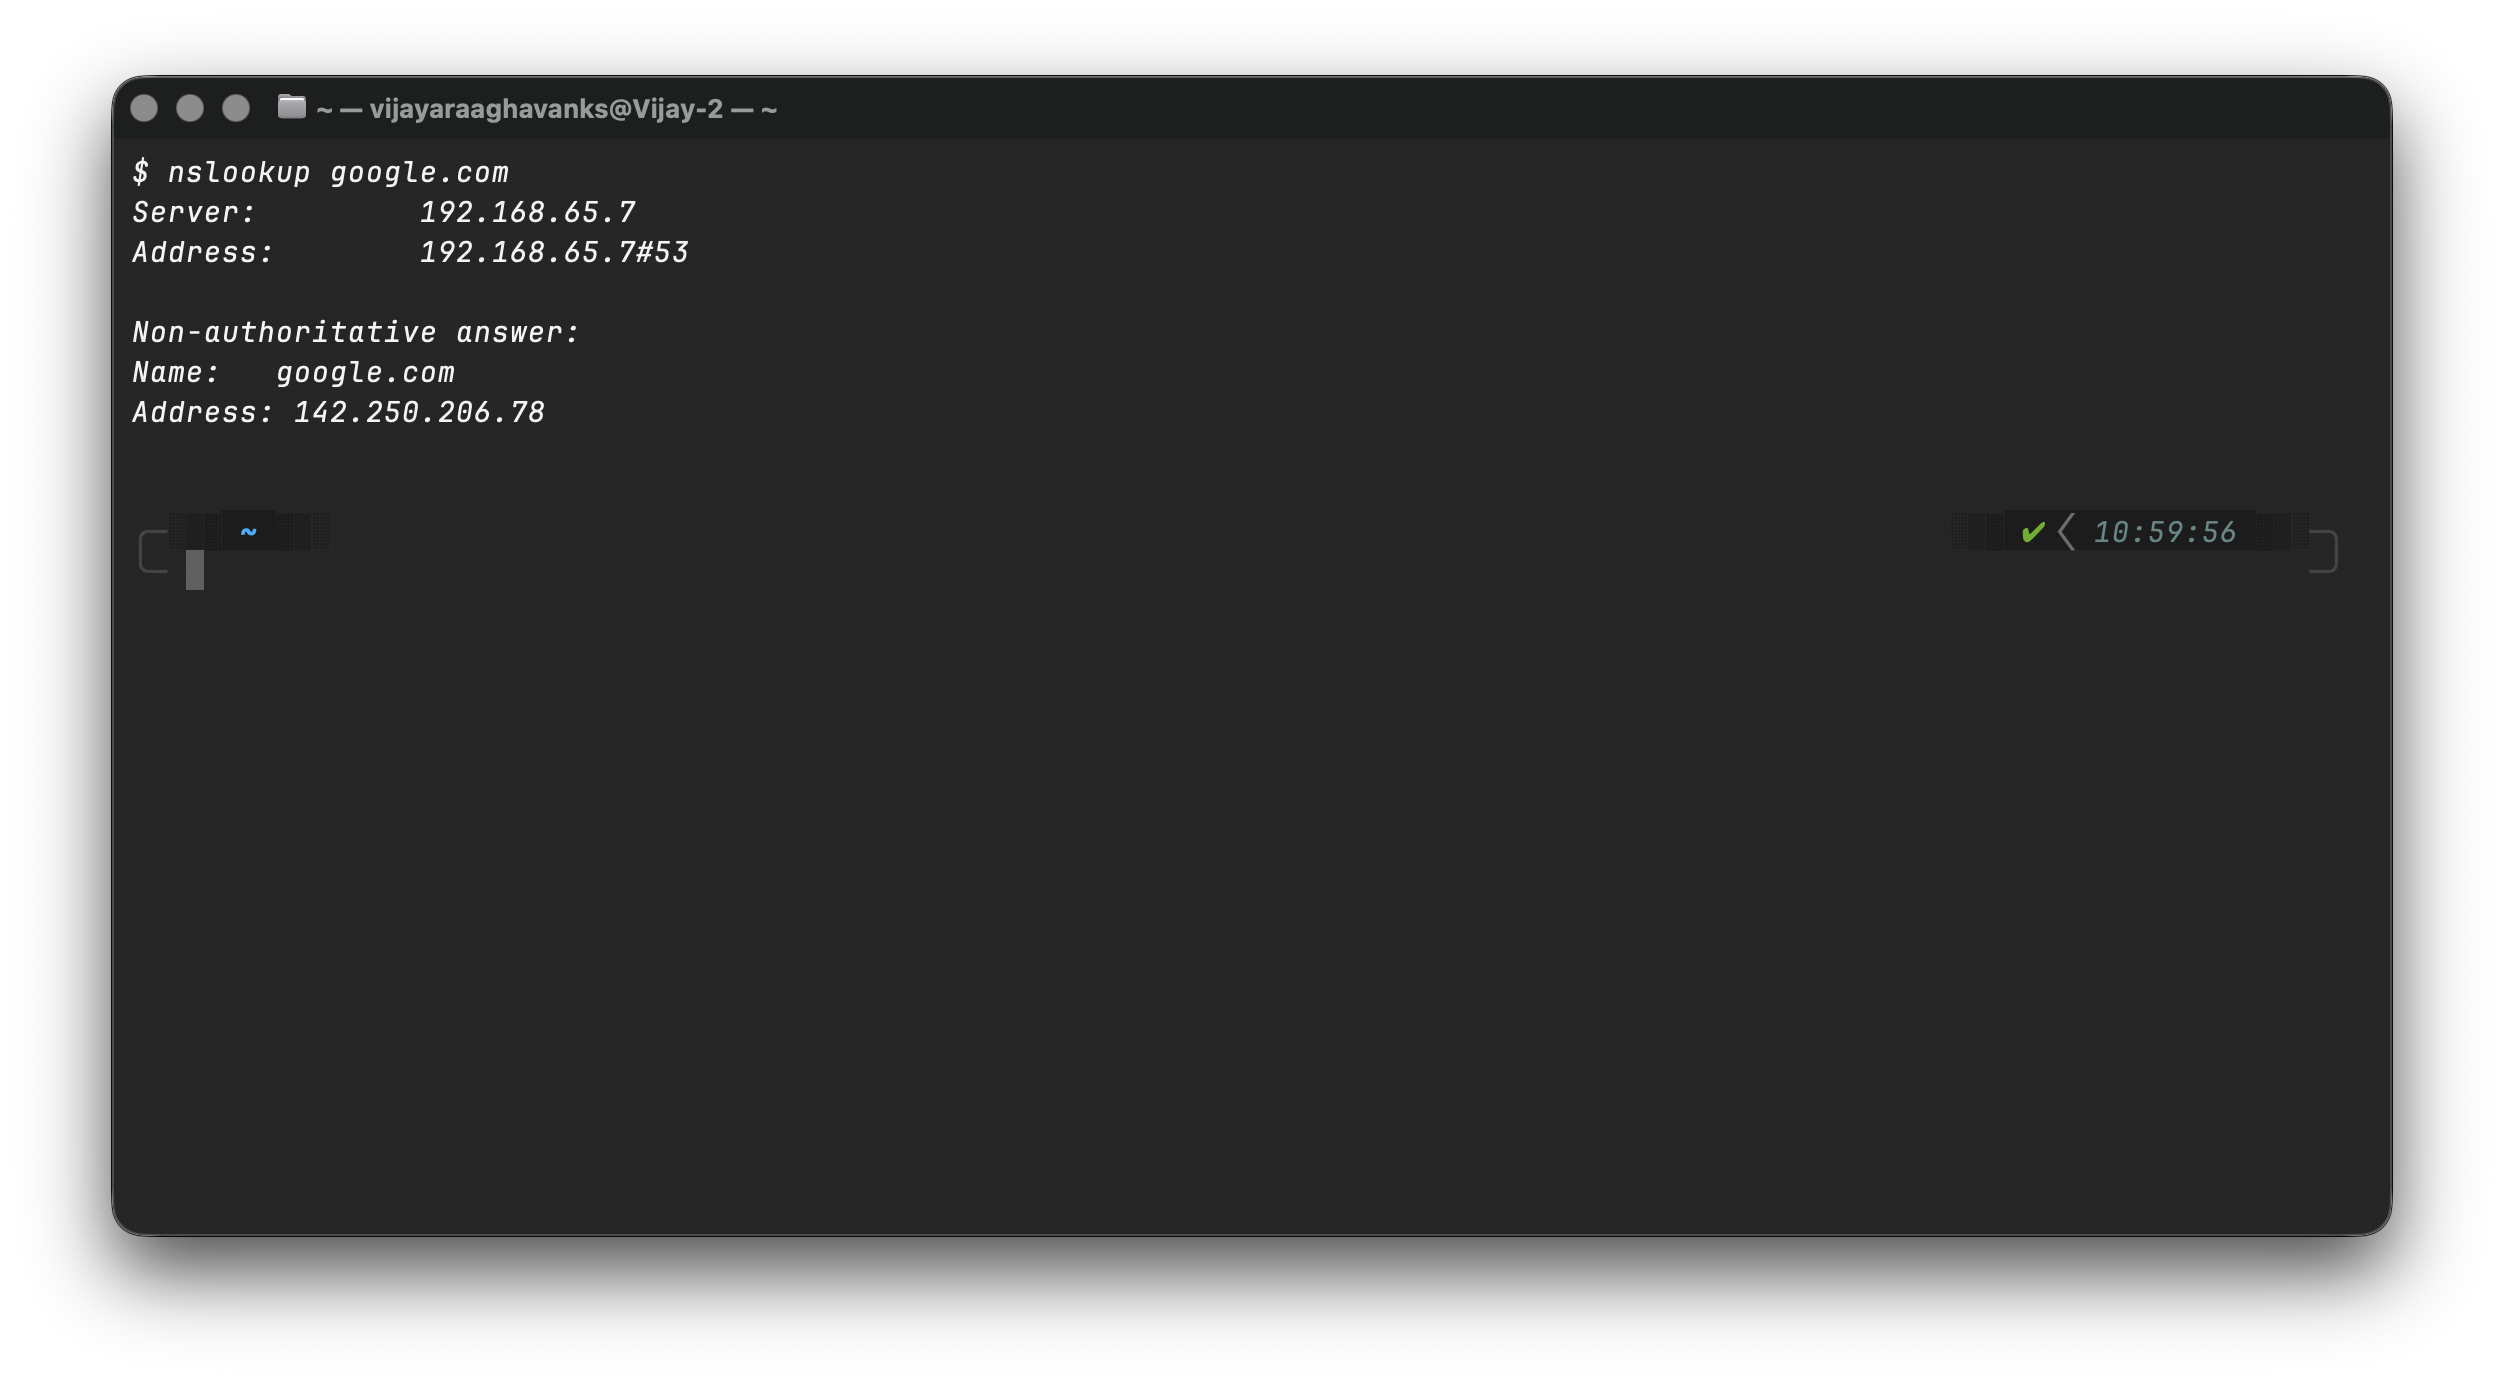
\includegraphics[width=0.8\linewidth]{screenshots/14_nslookup.png}\caption{nslookup google.com}\end{figure}

\subsection*{2.15 host -- simple DNS lookup utility}
\begin{lstlisting}[style=bashstyle]
$ host google.com
\end{lstlisting}
\texttt{host} is a lightweight DNS lookup tool. A single query returned both the domain's
\texttt{A} record (\texttt{142.250.206.78}) and its \texttt{MX} record
(\texttt{10 smtp.google.com}), demonstrating that \texttt{host} follows all record types for a
name by default rather than only \texttt{A} records.
\begin{figure}[h!]\centering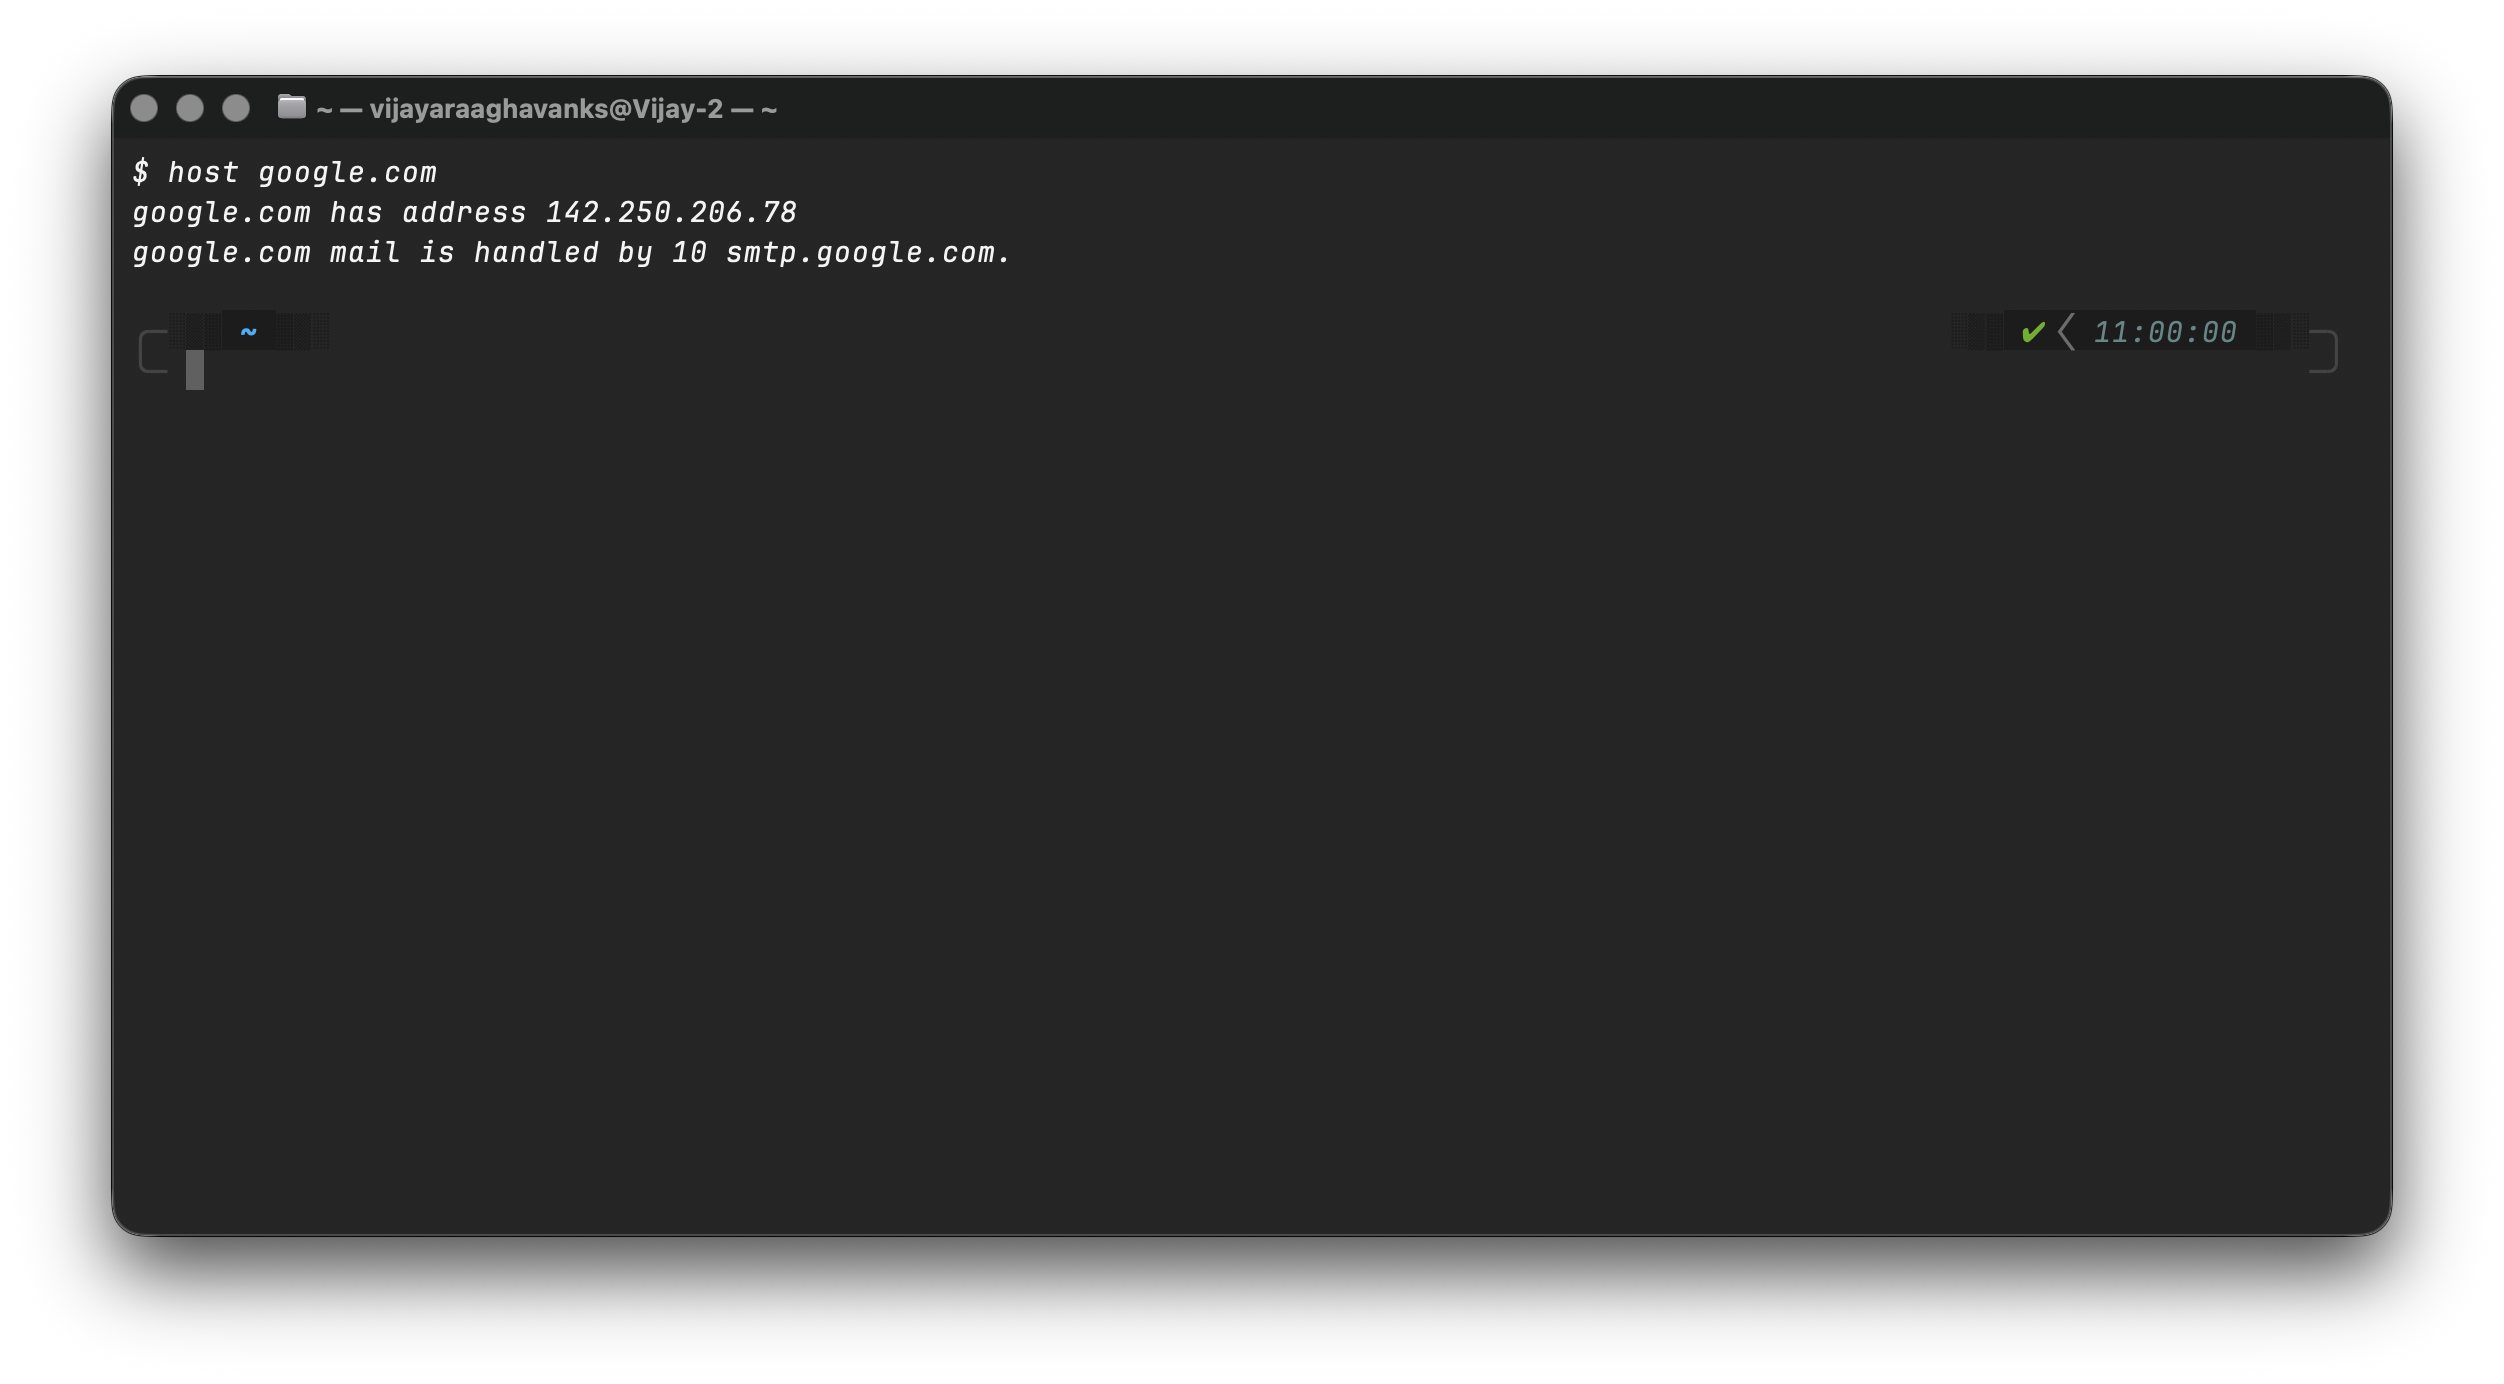
\includegraphics[width=0.8\linewidth]{screenshots/15_host.png}\caption{host google.com -- A and MX records}\end{figure}

\subsection*{2.16 whois -- domain registration lookup}
\begin{lstlisting}[style=bashstyle]
$ whois google.com
\end{lstlisting}
\texttt{whois} queries the registry/registrar's WHOIS database over TCP port 43 for domain
registration details. The response lists the registrar (MarkMonitor Inc.), creation date
(1997-09-15), expiry date (2028-09-14), name servers (\texttt{NS1--NS4.GOOGLE.COM}), and domain
status flags such as \texttt{clientTransferProhibited}.
\begin{figure}[h!]\centering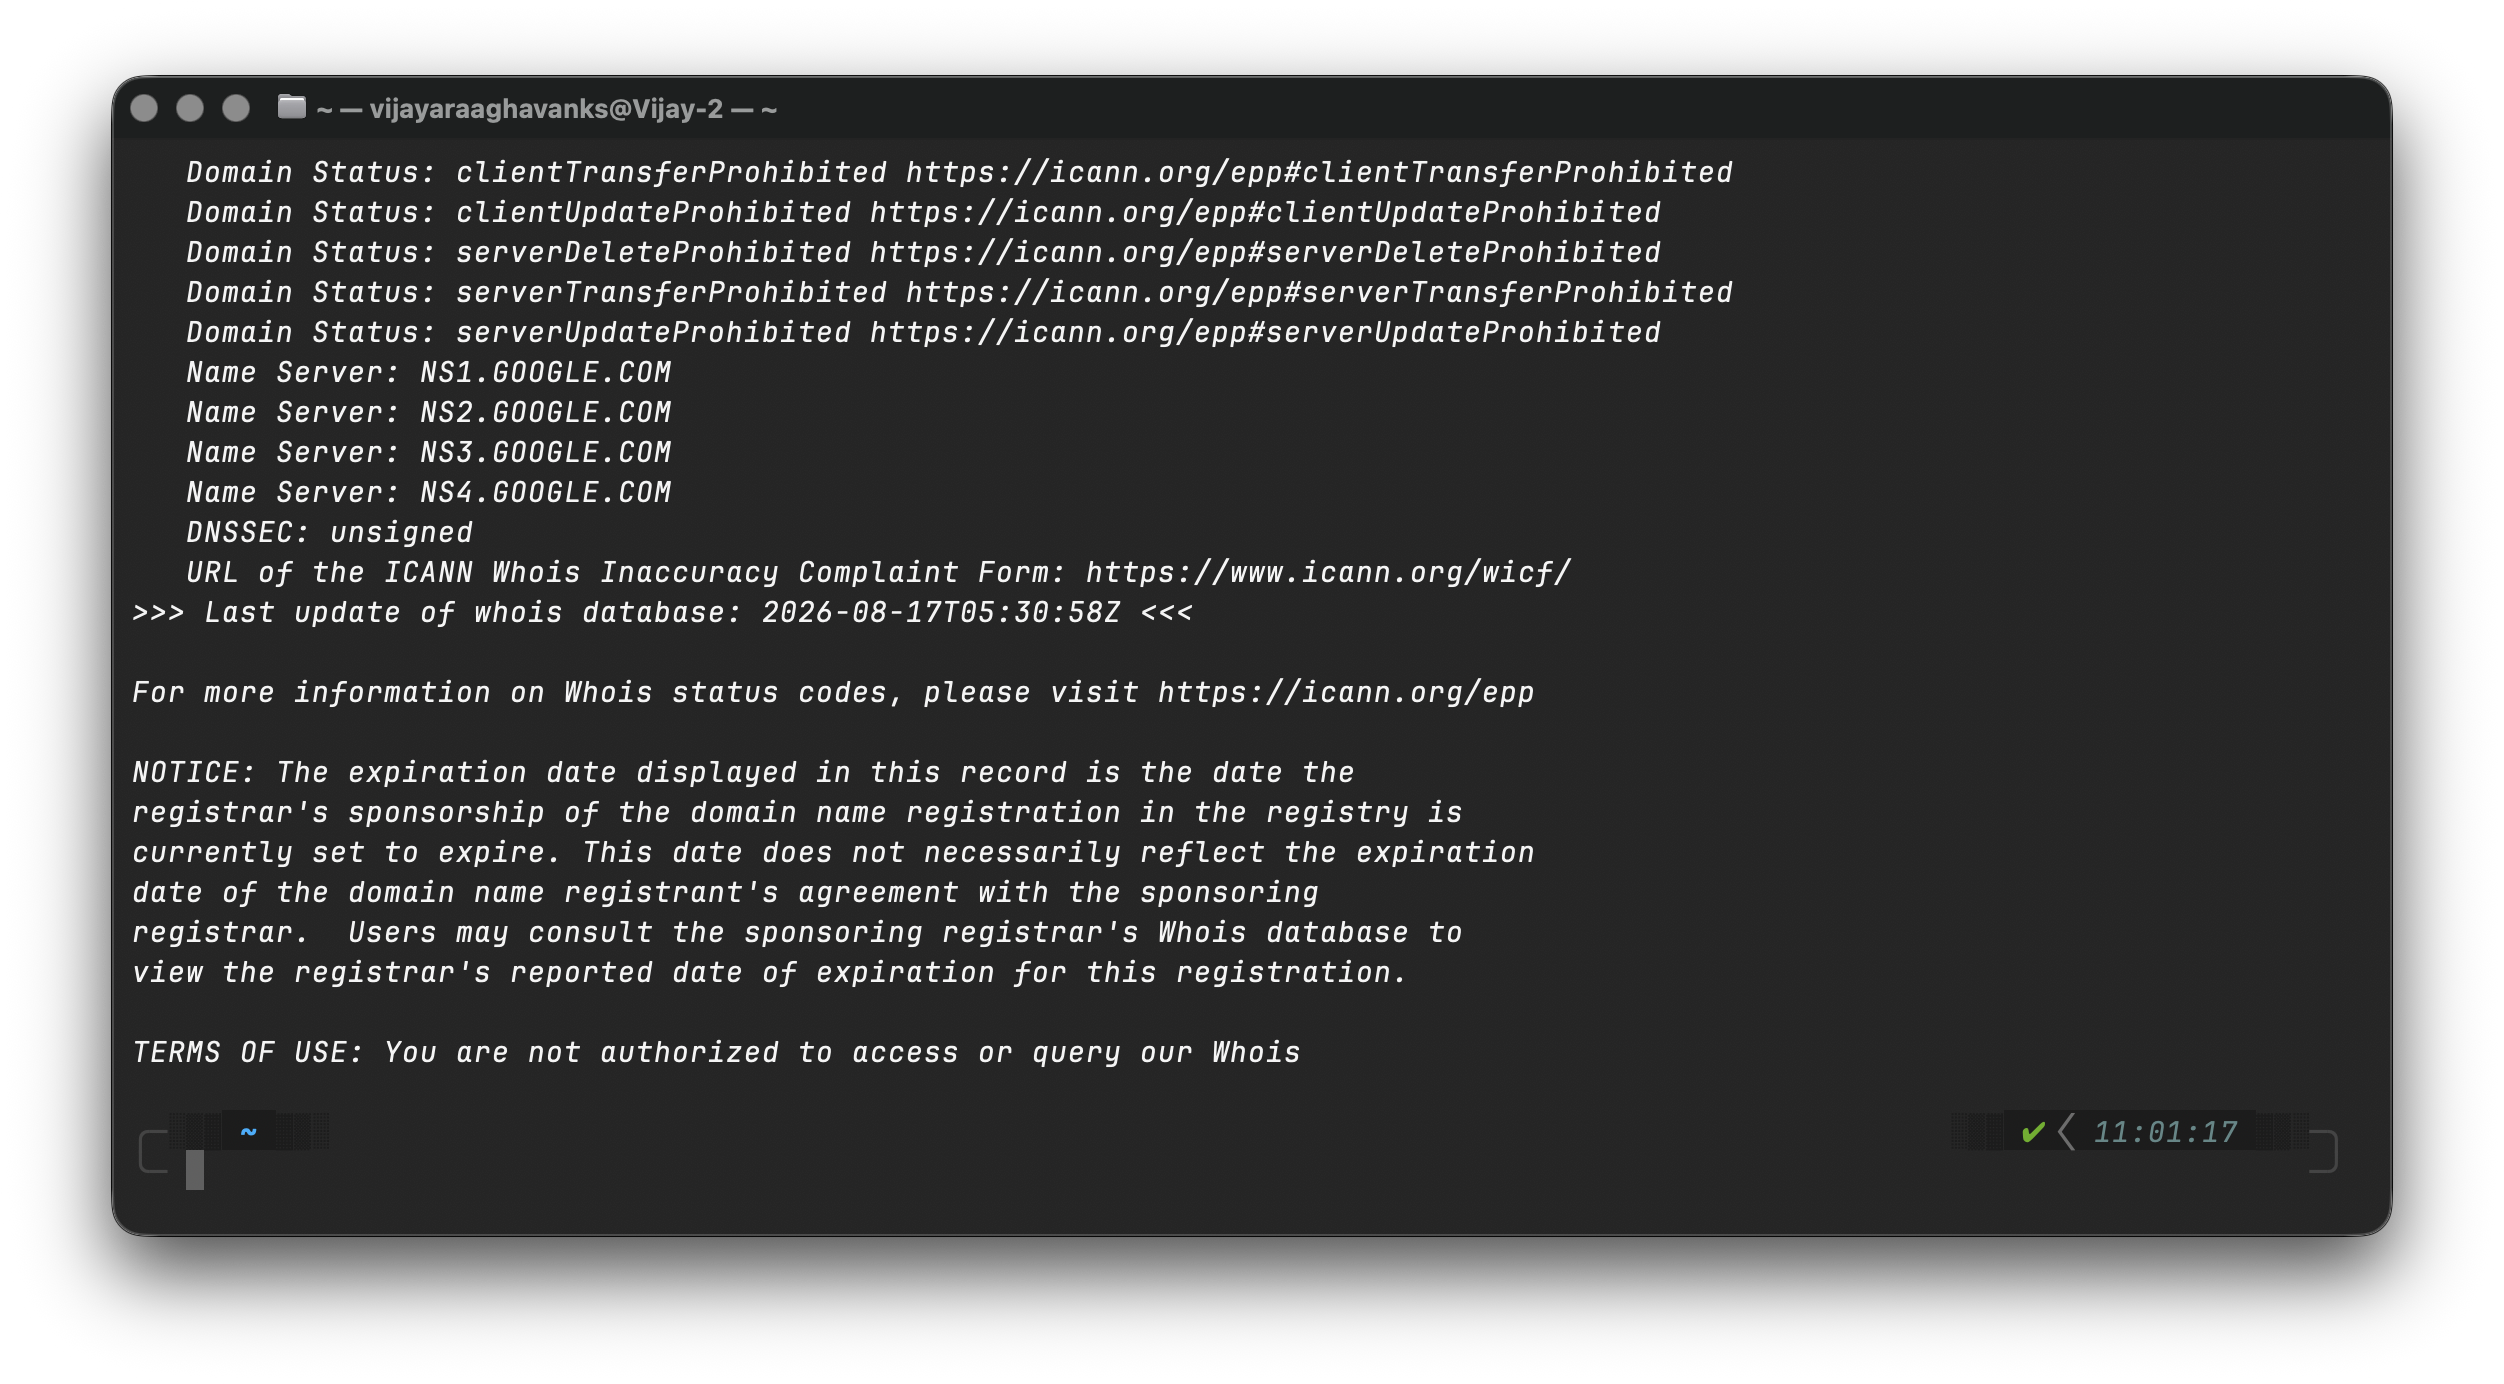
\includegraphics[width=0.8\linewidth]{screenshots/16_whois.png}\caption{whois google.com -- registrar and name-server details}\end{figure}

\clearpage
\section*{3. Part B -- Socket Programming System Calls}
The following POSIX/BSD socket API functions form the building blocks of TCP/IP and UDP
network programming in C. \texttt{socket()}--\texttt{bind()}--\texttt{listen()}--\texttt{accept()}
set up a TCP server; \texttt{connect()} is used by a TCP client; \texttt{send()}/\texttt{recv()}
(connection-oriented) and \texttt{sendto()}/\texttt{recvfrom()} (connectionless) exchange data;
the remaining functions handle byte-order conversion, name resolution, and socket
configuration.

\begin{longtable}{p{2.6cm}p{6.3cm}p{5.3cm}}
\toprule
\textbf{Function} & \textbf{Purpose \& Key Parameters} & \textbf{Return Value} \\
\midrule
\endhead
\texttt{socket()} & Creates an endpoint for communication. \newline
\texttt{int socket(int domain, int type, int protocol)} -- \texttt{domain}: \texttt{AF\_INET}/\texttt{AF\_INET6}; \texttt{type}: \texttt{SOCK\_STREAM} (TCP) / \texttt{SOCK\_DGRAM} (UDP). &
File descriptor on success, \texttt{-1} on error. \\
\texttt{bind()} & Assigns a local address (IP + port) to a socket. \newline
\texttt{int bind(int sockfd, struct sockaddr *addr, socklen\_t addrlen)}. Required before a server can \texttt{listen()}/\texttt{recvfrom()}. &
\texttt{0} on success, \texttt{-1} on error. \\
\texttt{listen()} & Marks a TCP socket as passive, ready to accept incoming connections, with a backlog queue. \newline
\texttt{int listen(int sockfd, int backlog)}. &
\texttt{0} on success, \texttt{-1} on error. \\
\texttt{connect()} & Initiates a connection (TCP) to a remote address, or fixes the peer address for a UDP socket. \newline
\texttt{int connect(int sockfd, struct sockaddr *addr, socklen\_t addrlen)}. &
\texttt{0} on success, \texttt{-1} on error. \\
\texttt{accept()} & Blocks until a connection request arrives on a listening socket; returns a new socket dedicated to that client. \newline
\texttt{int accept(int sockfd, struct sockaddr *addr, socklen\_t *addrlen)}. &
New connected socket fd, \texttt{-1} on error. \\
\texttt{close()} & Releases a socket (or any) file descriptor and its resources. \newline
\texttt{int close(int fd)}. &
\texttt{0} on success, \texttt{-1} on error. \\
\texttt{bzero()} & Zero-fills a block of memory (commonly used to clear a \texttt{sockaddr\_in} struct before populating it). \newline
\texttt{void bzero(void *s, size\_t n)}. &
None (void). \\
\texttt{htons()} & Converts a 16-bit value (e.g.\ port number) from Host byte order To Network byte order (big-endian). \newline
\texttt{uint16\_t htons(uint16\_t hostshort)}. &
The value in network byte order. \\
\texttt{htonl()} & Converts a 32-bit value (e.g.\ IPv4 address) from Host to Network byte order. \newline
\texttt{uint32\_t htonl(uint32\_t hostlong)}. &
The value in network byte order. \\
\texttt{ntohs()} & Converts a 16-bit value from Network byte order To Host byte order -- inverse of \texttt{htons()}. \newline
\texttt{uint16\_t ntohs(uint16\_t netshort)}. &
The value in host byte order. \\
\texttt{ntohl()} & Converts a 32-bit value from Network to Host byte order -- inverse of \texttt{htonl()}. \newline
\texttt{uint32\_t ntohl(uint32\_t netlong)}. &
The value in host byte order. \\
\texttt{read()} & Generic POSIX call to read bytes from any file descriptor, including a connected socket. \newline
\texttt{ssize\_t read(int fd, void *buf, size\_t count)}. &
Bytes read (\texttt{0} = EOF/peer closed), \texttt{-1} on error. \\
\texttt{write()} & Generic POSIX call to write bytes to any file descriptor, including a connected socket. \newline
\texttt{ssize\_t write(int fd, const void *buf, size\_t count)}. &
Bytes written, \texttt{-1} on error. \\
\texttt{send()} & Sends data on a \emph{connected} socket (TCP, or UDP after \texttt{connect()}), with socket-specific flags. \newline
\texttt{ssize\_t send(int sockfd, const void *buf, size\_t len, int flags)}. &
Bytes sent, \texttt{-1} on error. \\
\texttt{recv()} & Receives data from a connected socket. \newline
\texttt{ssize\_t recv(int sockfd, void *buf, size\_t len, int flags)}. &
Bytes received (\texttt{0} = peer closed), \texttt{-1} on error. \\
\texttt{sendto()} & Sends a datagram to an explicit destination address -- used by connectionless UDP sockets. \newline
\texttt{ssize\_t sendto(int sockfd, const void *buf, size\_t len, int flags, struct sockaddr *dest, socklen\_t addrlen)}. &
Bytes sent, \texttt{-1} on error. \\
\texttt{recvfrom()} & Receives a datagram and also fills in the sender's address -- the UDP counterpart of \texttt{recv()}. \newline
\texttt{ssize\_t recvfrom(int sockfd, void *buf, size\_t len, int flags, struct sockaddr *src, socklen\_t *addrlen)}. &
Bytes received, \texttt{-1} on error. \\
\texttt{select()} & Monitors multiple file descriptors, blocking until one becomes readable/writable or a timeout expires -- used for I/O multiplexing and implementing timeouts on blocking calls. \newline
\texttt{int select(int nfds, fd\_set *readfds, *writefds, *exceptfds, struct timeval *timeout)}. &
Number of ready descriptors, \texttt{0} on timeout, \texttt{-1} on error. \\
\texttt{setsockopt()} & Sets a configurable option on a socket, e.g.\ \texttt{SO\_REUSEADDR} to allow immediate rebinding of a port. \newline
\texttt{int setsockopt(int sockfd, int level, int optname, const void *optval, socklen\_t optlen)}. &
\texttt{0} on success, \texttt{-1} on error. \\
\texttt{fcntl()} & General file-descriptor control call; on sockets, commonly used to set non-blocking mode via \texttt{O\_NONBLOCK}. \newline
\texttt{int fcntl(int fd, int cmd, ...)}. &
Depends on \texttt{cmd} (often \texttt{0}/flags on success), \texttt{-1} on error. \\
\texttt{getpeername()} & Retrieves the address of the peer connected to a socket. \newline
\texttt{int getpeername(int sockfd, struct sockaddr *addr, socklen\_t *addrlen)}. &
\texttt{0} on success, \texttt{-1} on error. \\
\texttt{gethostname()} & Retrieves the standard host name of the local machine. \newline
\texttt{int gethostname(char *name, size\_t len)}. &
\texttt{0} on success, \texttt{-1} on error. \\
\texttt{gethostbyname()} & Resolves a host name to its IP address(es) (legacy API, superseded by \texttt{getaddrinfo()} but still widely used). \newline
\texttt{struct hostent *gethostbyname(const char *name)}. &
Pointer to \texttt{hostent} on success, \texttt{NULL} on error. \\
\texttt{gethostbyaddr()} & Performs a reverse lookup, resolving an IP address back to a host name. \newline
\texttt{struct hostent *gethostbyaddr(const void *addr, socklen\_t len, int type)}. &
Pointer to \texttt{hostent} on success, \texttt{NULL} on error. \\
\bottomrule
\end{longtable}

\section*{4. Learning Outcomes}
\begin{itemize}
  \item Gained hands-on familiarity with sixteen standard Linux networking diagnostic tools and
        learned which layer of the network stack each one operates on -- link/interface
        (\texttt{ifconfig}, \texttt{iwconfig}), network/routing (\texttt{route},
        \texttt{netstat -r}, \texttt{traceroute}, \texttt{tracepath}, \texttt{mtr}), transport/
        application reachability (\texttt{ping}, \texttt{nmap}), DNS (\texttt{dig},
        \texttt{nslookup}, \texttt{host}, \texttt{whois}), and raw packet capture
        (\texttt{tcpdump}).
  \item Learned to interpret \texttt{traceroute}/\texttt{tracepath}/\texttt{mtr} output in a
        NAT/containerised environment, and understood \emph{why} intermediate hops can appear as
        \texttt{*} even though end-to-end connectivity is fully functional -- an important
        distinction between "no route" and "ICMP diagnostic traffic filtered."
  \item Practised correlating live packet captures (\texttt{tcpdump}) with the higher-level
        tools that generated the traffic (\texttt{ping}, DNS resolution), reinforcing how ICMP
        and DNS operate at the packet level.
  \item Studied the complete socket API life cycle for both connection-oriented (TCP) and
        connectionless (UDP) communication, and understood why byte-order conversion functions
        (\texttt{htons}/\texttt{htonl}/\texttt{ntohs}/\texttt{ntohl}) are mandatory whenever
        multi-byte fields cross the network, given differing host endianness.
  \item Understood the role of auxiliary calls such as \texttt{select()} (multiplexing/timeout),
        \texttt{setsockopt()} (socket configuration) and \texttt{fcntl()} (non-blocking I/O) in
        building robust, production-quality socket applications beyond the basic
        \texttt{send}/\texttt{recv} loop.
\end{itemize}

\end{document}
